\documentclass[compress,aspectratio=169,10pt,usenames,dvipsnames]{beamer}

\mode<presentation>

\setbeamertemplate{theorems}[numbered]

\usetheme{CalPoly2023}

% use if you want greyed out steps rather than invisible
%\setbeamercovered{transparent}	

%Path relative to the main .tex file 
\graphicspath{ {./images} }

\usepackage{graphicx, amsmath, amsthm, amssymb, enumerate, esint, mathtools,multirow}
\usepackage{amsfonts,mathrsfs,float,array}
%\usepackage{xypic}
%\usepackage{tikz-cd}
\usepackage{tikz}
\usetikzlibrary{angles,quotes}
\usetikzlibrary{arrows, shapes, decorations}
\usepackage{tikz-3dplot}
%\usepackage{pgfplots}
%\usepackage{rotating}
%\usepackage[shortlabels]{enumitem}
\usepackage{subfigure}
\usepackage{multicol}
%\usepackage{amsmath}
%\usepackage{epsfig}
%\usepackage{graphicx}
%\usepackage[all,knot]{xy}
%\xyoption{arc}
\usepackage{url}
\usepackage{multimedia}
\usepackage{color}
%\usepackage[usenames,dvipsnames]{xcolor}

\definecolor{britishracinggreen}{rgb}{0.0, 0.26, 0.15}
\definecolor{bluegray}{rgb}{0.4, 0.6, 0.8}
\definecolor{lightgray}{rgb}{0.83, 0.83, 0.83}
\definecolor{pastelred}{rgb}{1.0, 0.41, 0.38}
\definecolor{wildwatermelon}{rgb}{0.99, 0.42, 0.52}
\definecolor{classicrose}{rgb}{0.98, 0.8, 0.91}
\definecolor{cobalt}{rgb}{0.0, 0.28, 0.67}
\definecolor{columbiablue}{rgb}{0.61, 0.87, 1.0}

\newtheorem{prop}[theorem]{Proposition}
\newtheorem{conj}[theorem]{Conjecture}
\newcommand{\Z}{\mathbb{Z}}
\newcommand{\R}{\mathbb{R}}
\newcommand{\N}{\mathbb{N}}
\newcommand{\C}{\mathbb{C}}
\newcommand{\Q}{\mathbb{Q}}

\addtobeamertemplate{navigation symbols}{}{%
    \usebeamerfont{footline}%
    \usebeamercolor[fg]{footline}%
    \hspace{1em}%
    {\footnotesize \insertframenumber/\inserttotalframenumber}
}

\title[Thesis Defense]{Applications of Representation Theory to Braids and Anyonic Systems \\ \;}
\author[Jaxon Green]{Jaxon Green}
\institute[Cal Poly]{}%{California Polytechnic State University} 
\date{August 30, 2024}
\setbeamercolor{section}{use=structure,fg=CPwhite,bg=CPgreen}
\setbeamercolor{section in head/foot}{use=structure,fg=CPwhite,bg=CPgreen}
\setbeamercolor{block title}{use=structure,fg=CPwhite,bg=CPgreen}
\setbeamercolor{block body}{use=structure,fg=black,bg=CPbeige}

\useoutertheme[subsection=false]{smoothbars}

\listfiles
\begin{document}

\begin{frame}
	\titlepage
\end{frame}

\begin{frame}
	\textbf{Outline}
	\begin{enumerate}
		\item Introduction to Representation Theory
		\item $SO(2)$: The Rotation Group in Two Dimensions
		\item $SO(3)$: The Rotation Group in Three Dimensions
		\item Euclidean Groups
		\item Lorentz and Poincar\'e Groups
		\item Braid Group and Anyons
	\end{enumerate}
\end{frame}


\section{Introduction to Representation Theory}
\begin{frame}
	\sectionpage
\end{frame}


\begin{frame}
	\vfill
	\begin{block}{Question}
		How does one study a mathematical structure? (Sets, Groups, Vector Spaces, etc.)
	\end{block}
	\vfill

	\onslide<2->
	\begin{block}{Answer}
		By studying its maps!
	\end{block}
	
	\vfill
\end{frame}

\begin{frame}
	\vfill
	\begin{block}{}
		Maps help us to identify unknown structures with understood ones.
	\end{block}
	\vfill
	\begin{example}
		Cayley's Theorem: $\phi: G \rightarrow S_G$
	\end{example}
	\vfill
	\onslide<2->
	\begin{block}{}
		Maps help us to make connections that are otherwise unintuitive.
	\end{block}
	\vfill
	\begin{example}
		$(0,1)$ is isomoprhic to $\R$.
	\end{example}
	\vfill
%\end{frame}
%
%
%\begin{frame}
%	\vfill
	\onslide<3->
	\begin{block}{}
		In this thesis, we look to understand the behavior of groups through the lens of a special kind of map.
	\end{block}
	\vfill
\end{frame}

\begin{frame}
	\vfill
	\begin{definition}
	 Let $G$ be a group. A \textbf{representation} of degree $n$ is a group homomorphism that maps a $G$ into $GL_n(\mathbb{C}).$
	$$\phi:G\rightarrow GL_n(\mathbb{C})$$
	\end{definition}
	\vfill	
	We say that $\phi$ is a representation of $G$. 
	\vfill
	If $\phi$ is an injective homomorphism, we say that the representation is \textbf{faithful}. Otherwise, the representation is called \textbf{degenerate}.
	\vfill
\end{frame}


\begin{frame}
	\vfill
	\begin{block}{Question}
		What is so special about representations?
	\end{block}
	\vfill
	\onslide<2->
	\begin{block}{Answer}
		Matrices are some of the most well-understood strucutres in all of mathematics. We can use linear algebra to gain insight into group properties.
	\end{block}
\end{frame}

\begin{frame}
\vfill
\begin{example}
Let $G$ be the group of all roots of unity (under multiplication). Explicitly, $G=\{e^{\frac{2\pi im }{n}}\mid m,n\in\Z\}$. One representation can be created by
\vfill
	\renewcommand{\arraystretch}{1.25}

$$\phi:G\rightarrow GL_2(\mathbb{C})$$%\\
		%$\hspace{0mm}
$$e^{2\pi i\frac{m}{n}}\mapsto \begin{bmatrix}
							\cos(\frac{2\pi m}{n}) & \sin(\frac{2\pi m}{n}) \\
							-\sin(\frac{2\pi m}{n}) & \cos(\frac{2\pi m}{n})
						      \end{bmatrix}$$\\
\end{example}
\vfill
This representation is degree $2$ and is degenerate.
\vfill
\end{frame}


\begin{frame}
\vfill
There is another equivalent definition for representations:
\vfill
\begin{definition}
	Let $G$ be a group, $V$ be an $n$-dimensional vector space, and let $\mathcal{L}(V)$ be the group of linear operators on $V$ under composition. A \textbf{representation} of $G$ of degree $n$ is a group homomorphism that maps the $G$ into $\mathcal{L}(V)$
$$\phi: G \rightarrow \mathcal{L}(V) $$
\end{definition}
\vfill

We identify matrices in $GL_n(\C)$ with matrices of operators in $\mathcal{L}(V)$.
\vfill
We will switch between definitions when useful
\vfill
\end{frame}

\begin{frame}
\vfill
\begin{example}
	Let $G$ be the complex unit circle ($G=\{e^{i\theta} \mid \theta\in[0,2\pi)\}$) and the operation of multiplication and let $V = \mathbb{C}$. Then, 
$$\phi:G\rightarrow \mathcal{L}(V)$$
$$e^{i\theta}\mapsto U_{e^{i\theta}}$$
where $U_{e^{i\theta}}:\C \rightarrow \C$ such that $U_{e^{i\theta}}(re^{i\psi}) = e^{i\theta}re^{i\psi}$ $\forall re^{i\psi}\in G$
\end{example}
\vfill
Depending on $V$, this is either a one or two degree representation. It is faithful.
\end{frame}
%
%
\begin{frame}
\vfill
\begin{block}{Question}
	When are two representations representing the same information?
\end{block}
\vfill
\onslide<2->
\begin{definition}
	Two representations, $\phi$ and $\psi$, are said to be \textbf{equivalent representations} if there exists some invertible operator/matrix (depending on definition of representation), $M$, such that $$\phi = M \psi M^{-1}$$
\end{definition}
\vfill
Representation equivalence (conjugation) is an equivalence relation.
\vfill
This is directly related to similarity transformations and matrix canonical forms.
\vfill
\end{frame}
%
%
\begin{frame}
\vfill
We can detect matrix similarity with the following operation:
\vfill
\begin{definition}
	The \textbf{character} of a representation, $\phi$, on $g \in G$, denoted $\chi^{\phi}(g)$, is defined by $$\chi^{\phi}(g)=trace(\phi(g))$$
\end{definition}
\vfill
The trace operation satisfies $trace(AB)=trace(BA)$ for any two matrices.
\vfill
\begin{theorem}
	If two representations are equivalent, then character of both representations are the same.
\end{theorem}
\vfill
\end{frame}
%
%
\begin{frame}
\vfill
Much like in the study of linear algebra, we will explore the decomposition of representations into its invariant components
\vfill
\begin{definition}
	Let $\phi$ be a representation of the group $G$ and $\phi(G) \coloneq \{\phi(g)=\phi_g: V\rightarrow V \hspace{1mm}| \hspace{1mm} g\in G\}$. Let $W \subset V$. $W$ is said to be an \textbf{invariant subspace} with respect to $\phi(G)$ if $\forall v \in W$ and $\forall g \in G$, $\phi_g(v)\in W$.
\end{definition}
\vfill
\begin{definition}
	A representation is said to be \textbf{irreducible} if there is no nontrivial, invariant subspace with respect to it. Otherwise, we say that the representation is reducible.
\end{definition}
\vfill
We look to the the eigendecomposition of matrices of a representation to find such subspaces.
\end{frame}
%
%
\begin{frame}
\vfill
In order to be more explicit in our discussion, we introduce new notation:
\vfill
\begin{definition}
	If $M$ and $N$ are square matrices, then let $$M\oplus N \coloneq \begin{bmatrix}
																			M & 0\\
																			0 & N\\
																		\end{bmatrix}$$
	we call this new matrix the \textbf{direct sum} of M and N.
\end{definition}
\vfill
\begin{example}
$$\begin{bmatrix}
	1 & 0 & 0 \\
	0 & 1 & 0 \\
	0 & -1 & -1
\end{bmatrix} = \begin{bmatrix}
					1
					\end{bmatrix} \oplus
					\begin{bmatrix}
						1 & 0 \\
						-1 & -1
					\end{bmatrix}$$
\end{example}
\vfill
\end{frame}
%
%
\begin{frame}
\vfill
Following our natrual inclination, we can use our notion of block-diagonal matrix decompositions to explicitly characterize representations.
\vfill
\begin{theorem}
	Let $\phi$ be a representation of a group $G$.  Then there exists a set of irreducible representations of $G$, $\{\psi_i\}_{i=1}^j$, such that $$\phi = T\left(\bigoplus_{i=1}^j \alpha_i*\psi_i\right)T^{-1}$$ where $\alpha_i*\psi_i \coloneq \underbrace{\psi_i \oplus \psi_i \oplus \hdots \oplus \psi_i}_{\alpha_i times}$ and $T$ is some invertible matrix/operator. 
\end{theorem}
\vfill
We prove this theorem using induction on the degree of representation.
\vfill 
The results of this theorem show us that we can completely characterize any representation in terms of its irreducible components. With this in mind, we can characterize important properties of irreducible representations
\vfill
\end{frame}
%
%
\begin{frame}
\vfill

\begin{theorem} \textbf{Schur's Theorem:}
	Let $\phi$ and $\psi$ be two irreducible representations of the group $G$. Let $M$ be a matrix defined such that $M\phi(g) = \psi(g)M \hspace{1.5mm}\forall g \in G$. Then $M$ is invertible or $0$. 
\end{theorem}
\vfill
Schur's Theorem tells us that irreducible representations are either completely unrelated or equivalent, much like eigenspaces.
\vfill
\end{frame}

\begin{frame}
\vfill
\begin{theorem}
	Let $\phi$ be an irreducible representation and $M$ be a matrix/operator such that $M\phi(g)=\phi(g)M \hspace{1.5mm}\forall g \in G$. Then $M$ is a mulptiple of the identity matrix/map.
\end{theorem}
\vfill
This identity will be incredibly useful for finding representations when we know that certain matrices will commute.
\vfill
\end{frame}

\begin{frame}
\vfill
\begin{theorem}
If $G$ is an abelian group, then any irreducible representation of $G$ can be viewed as a degree one representation.
\end{theorem}
\vfill
This identity trivializes the classification of abelian groups, giving their representations complete sets of eigenvalues.
\end{frame}
%
%
\begin{frame}
\vfill
Irreducible representations are not the only special kind of representation. When $V$ is an inner-product space, we have more structure.
\vfill
\begin{definition}
	Let $V$ be an inner-product space. Let $U \in \mathcal{L}(V)$. $U$ is said to be \textbf{unitary} if $U$ is surjective and $\forall x,y \in V$, $\langle x , y \rangle = \langle U(x) , U(y) \rangle$.
\end{definition}
\vfill
\begin{definition}
	A representation, $\phi$, of a group, $G$, is said to be a \textbf{unitary representation} if $\forall g\in G$, $\phi(g)$ is unitary.
\end{definition}
\vfill
\end{frame}

\begin{frame}
\vfill
\begin{theorem}
	Every representation of a finite group on an inner-product space is equivalent to a unitary representation
\end{theorem}
\vfill
The above theorem gives us the utility of being able to tranform any representation into its unitary form. We can make our irreducible representations unitary as well.
\vfill
When we consider the unitary irreducible representations of a group, we can make striking conclusions.
\end{frame}
%
%
\begin{frame}
\vfill
\begin{theorem}
	Let $G$ be a finite group, let $\Phi$ be the set of distinct (inequivalent to others in set) irreducible, unitary representation of $G$. Let $\phi,\psi \in \Phi$ with degrees $n_{\phi}$ and $n_{\psi}$ respectively. Let $\phi_g \coloneq \phi(g)$ and $\psi_g \coloneq \psi(g)$. Then the following equality holds:
$$\frac{n_\phi}{|G|} \sum_{g\in G} \left[\phi_g \right]_{ij} \left[\psi_g^\dag \right]_{kl} = \begin{cases}
																						1 & \text{if } \psi = \phi,\hspace{1mm} j=k,\hspace{1mm} \text{and } i=l\\
																						0 & else
																					 \end{cases}$$
where for any matrix $M=\left[m\right]_{ij}$, $\left[M^\dag\right]_{ij} = \overline{m}_{ji} $. We refer to this as the \textbf{orthonormality condition} of unitary irreducible representations.
\end{theorem}
\vfill
There is no doubt complexity here, but this theorem can be made more digestible.
\vfill
\end{frame}
%
%
\begin{frame}
\vfill
We create a $|G|$-dimensional vector space in the following way: For fixed $\phi,i,j$,
$$\sqrt{\frac{n_\phi}{|G|}}\left([\phi_{g_1}]_{ij},\hspace{1mm} [\phi_{g_2}]_{ij}, \hspace{1mm}\hdots \hspace{1mm},\hspace{1mm} [\phi_{g_{|G|}}]_{ij}\right)$$
\vfill
Then, $\frac{n_\phi}{|G|} \sum_{g\in G} \left[\phi_g \right]_{ij} \left[\psi_g^\dag \right]_{kl}$ is just an inner product of vectors in this space. 
\vfill
Further,
$$\begin{cases}
																						1 & \text{if } \psi = \phi,\hspace{1mm} j=k,\hspace{1mm} \text{and } i=l\\
																						0 & else
																					 \end{cases}$$ is the conclusion that these vectors are orthonormal to one another in choice of $\phi,i,$and $j$.
\vfill
\end{frame}
%
%
\begin{frame}
\vfill
We have a another very similar property that unitary irreducible representations meet:
\vfill
\begin{theorem}
	Let $G$ be a finite group, let $\Phi = \{\phi \mid \phi$ is a unitary, irreducible representation of $G\}$, and let $n_\phi$ denote the degree of the representation $\phi$. Then for any pair $g$, $h \in G$, 
$$\sum_{\phi \in \Phi} \sum_{i=1}^{n_\phi} \sum_{j=1}^{n_\phi} \frac{n_\phi}{|G|} \left[\phi_g\right]_{ij}\left[\phi_{h}^\dag\right]_{ji} = \begin{cases}
																										1 & if \hspace{1mm} g = h \\
																										0 & else
																									\end{cases}$$
This is referred to as the \textbf{completeness condition} of unitary, irreducible representations.
\end{theorem}
\vfill
Here, we mean complete in the sense that our irreducible unitary decomposition is a complete characterization of a generic repesentation. 
\vfill
\end{frame}

\begin{frame}
This is a consequence of the follwoing relationship we derive from the previous theorem:
\vfill
\begin{theorem}
	For any finite group, $G$, $\sum_{\phi \in \Phi} n_\phi^2 = |G|$ where $\Phi$ is the set of a distinct, irreducible representations of $G$.
\end{theorem}
\vfill
Here, we see that for any finite group, there is a finite set of irreducible representations that we can decompose generic representations into.
\vfill
\end{frame}
%
%
\begin{frame}
\vfill
Generalizing the properties of unitary representations to groups with infinite order requires more careful construction (Haar Measure).
\vfill
Generalizing representation theory to infinite-dimensional vector spaces also requires care, but we can explictly approach this
\vfill
\begin{definition}
	A \textbf{matrix element} of a representation $\phi$ of a group $G$ on a inner-product space $V$ is a function defined in the following way:
$$f:G\rightarrow\C$$
$$g\mapsto\langle\phi(g)v,w\rangle$$
for some fixed $v,w\in V$.
\vfill
\end{definition}
\vfill
\end{frame}
%
%
\begin{frame}
\vfill
When $V$ is finite-dimensional, then the choice of standard basis vectors gets us matrix entry.
\vfill
When we define representations on infinite-dimensional vector spaces, we will identify them by their matrix elements on orthonormal bases.
\vfill
\end{frame}

\begin{frame}
\vfill
We further generalize our notion of representations:
\vfill
\begin{definition}
	A \textbf{multi-valued representation} is a multi-valued mapping of a group into $GL_n(\C)$ which is a group homomorphism in the sense that at least one of the outputs (from each input) may be used to satisfy the homomorphism property.
\end{definition}
\vfill
$2$-valued representations will be of interest to us.
\vfill
\end{frame}
%
%
\section{$SO(2)$: The Rotation Group in Two Dimensions}

\begin{frame}
	\sectionpage
\end{frame}

\begin{frame}
\vfill
$SO(2)$ is a group whose elements correspond to the action of rotating vectors in two-dimensional space about some central point. 
\vfill
For our discussion, we will take vectors to be in $\R^2$, rotations occuring counterclockwise about the origin. 
\vfill
Angle measurement will be real-valued.
\vfill
We will take $\{e_1,e_2\}$ to be the standard basis of $\R^2$.
\vfill
\end{frame}
%
%
\begin{frame}
\vfill
If we let $(x,y)\in\R^2$ be rotated by $\theta$ into $(x',y')$, we can visualize it in the following way:
\vfill
\begin{figure}[H]
	\centering
	\begin{tikzpicture}[scale=0.7]
	                %\draw[step=1cm ,color=gray] (-4,-4) grid (4,4);
			\draw[thin,<->] (-4.1,0) -- (4.1,0) node[anchor=north west] {$e_1$};
			\draw[thin,<->] (0,-4.1) -- (0,4.1) node[anchor=south west] {$e_2$};
			\draw[fill=black] (0,0) coordinate (o);
			\draw[thick, ->] (0,0) -- (2,3) coordinate (a) node[anchor=south west] {$(x,y)$};
			\draw[thick, ->] (0,0) -- (-3,2) coordinate (b) node[anchor=south] {$(x',y')$};
			\pic [draw, ->, angle eccentricity=0.7, angle radius=0.8cm, "$\theta$"]{angle=a--o--b};
	\end{tikzpicture}
	\caption{Rotation of a generic vector in $\R^2$ by angle $\theta$}
\end{figure}
\vfill
\end{frame}
%
%
\begin{frame}
\vfill
If we identify each point with its polar coordinates, we can make a direct calculation for $(x',y')$:
\vfill
\begin{equation}
	\begin{aligned}
		x' &= x\cos(\theta) -y\sin(\theta)
	\end{aligned}
\end{equation}
\begin{equation}
	\begin{aligned}
		y' &= x\sin(\theta) +y\cos(\theta)
	\end{aligned}
\end{equation}
\vfill
\end{frame}
%
%
\begin{frame}
\vfill
Or alternatively
\vfill
\begin{equation}
	\begin{aligned}
		\begin{bmatrix}
			x' \\
			y'
		\end{bmatrix} &=
		\begin{bmatrix}
			\cos(\theta) & -\sin(\theta) \\
			\sin(\theta) & \cos(\theta)
		\end{bmatrix}
		\begin{bmatrix}
			x \\
			y
		\end{bmatrix}
	\end{aligned}
\end{equation}
\vfill
If we take all matrices of this form, we can verify that they form a group under matrix multiplication.
\vfill
We exercise care to ensure that we identify each rotation (modulo $2\pi$) with its corresponding matrix to show equivalence. The resulting group is $SO(2)$.
\end{frame}
%
%
\begin{frame}
\vfill
We can discuss some properties of $SO(2)$ matrices. Generally, we reference these matrices as $R(\theta)$
\vfill
\begin{theorem}
	For any $R(\theta)\in SO(2)$, $R(\theta)$ is an orthogonal matrix.
$$R(\theta)R(\theta)^\intercal=I_n$$
\end{theorem}
\vfill
\begin{theorem}
	For any $\theta$, $R(\theta)$ is a special matrix.
 $$\det(R(\theta))=1$$
\end{theorem}
\vfill
Hence, the group is entitled the \textbf{special orthogonal group (in two dimensions)}
\end{frame}
%
%
\begin{frame}
\vfill
$SO(2)$ is also a special type of group called a Lie group.
\vfill
\begin{definition}
	A \textbf{Lie Group} is a group that is a finite-dimensional smooth manifold in which the operations of multiplication and inversion are differentiable.
\end{definition}
\vfill
Intuitively, varying the parameter of $\theta$ varies group elements smoothly. We can use this principle to construct a "generator" of sorts.
\vfill
\end{frame}
%
%
\begin{frame}
\vfill
If we consider what the rotation matrix would be for an arbitrarily small angle, $d\theta$, we can write 
\vfill
\begin{equation}
	\begin{aligned}
		R(d\theta) \coloneq I_2 + (-i)d\theta  J
	\end{aligned}
\end{equation}  
\vfill
where the factor of $-i$ is conventionally use.
\vfill
$R(d\theta)$ differes from the identity matrix by a factor of $d\theta$.
\end{frame}
%
%
\begin{frame}
\vfill
This realization gives us two ways to calculate the instantaneous change after rotating by angle $\theta$.
\vfill
\begin{equation}
	\begin{aligned}
		R(\theta + d\theta) = R(\theta) - id\theta R(\theta)J
	\end{aligned}
\end{equation}  
\begin{equation}
	\begin{aligned}
		R(\theta + d\theta) = R(\theta) + \frac{d}{d\theta}R(\theta)d\theta
	\end{aligned}
\end{equation}  
\vfill
Putting both equations gives us a differential equation solved by
\vfill
\begin{equation}
	\begin{aligned}
		R(\theta) = e^{-i\theta J} = \sum_{n=0}^\infty \frac{(-i\theta J)^n}{n!}
	\end{aligned}
\end{equation}  
\vfill
\end{frame}
%
%
\begin{frame}
\vfill
We can explicitly solve our equation for $J$ by taking (4) explictly
\vfill
\begin{equation}
	\begin{aligned}
		\begin{bmatrix}
			1 & 0 \\
			0 & 1
		\end{bmatrix} + (-i)d\theta * \begin{bmatrix}
			j_{11} & j_{12} \\
			j_{21} & j_{22}
		\end{bmatrix} = R(d\theta) = \begin{bmatrix}
			\cos(d\theta) & -\sin(d\theta) \\
			\sin(d\theta) & \cos(d\theta)
		\end{bmatrix} = 
		\begin{bmatrix}
			1 & -d\theta \\
			d\theta & 1
		\end{bmatrix}
	\end{aligned}
\end{equation}
\vfill
To get
\vfill
\begin{equation}
	\begin{aligned}
		J = \begin{bmatrix}
			0 & -i \\
			i & 0
		\end{bmatrix}
	\end{aligned}
\end{equation}
\vfill
While $J$ is not in the group, it still is referred to as the generator of $SO(2)$ due to (7).
\end{frame}
%
%
\begin{frame}
\vfill
Now that we have characterized the group $SO(2)$ we can find its irreducible representations. 
\vfill
$SO(2)$ is abelian, so all irreducible representations are degree one.
\vfill
We look to the invariant subspaces of our generator for motivation.
\end{frame}
%
%
\begin{frame}
\vfill
If $\lambda$ is an eigenvalue of $J$, then $e^{-i\theta\lambda}$ is an eigenvalue of $R(\theta)$.
\vfill
\begin{equation}
	\begin{aligned}
		R(\theta) (v) = \left(\sum_{i=0}^\infty \frac{(-i\theta J)^n}{n!}\right) (v) = \left(\sum_{i=0}^\infty \frac{(-i\theta \lambda)^n}{n!}\right)v = \left(e^{-i\theta \lambda}\right)v
	\end{aligned}
\end{equation}
\vfill
We place a restriction on our eigenvalue possibilities in order to appeal to the physical constraint:
\begin{equation}
	\begin{aligned}
		e^{-i2\pi n\lambda} = 1 \Rightarrow \lambda \in \Z
	\end{aligned}
\end{equation}
\vfill
Making $\lambda\in\Z$.

\end{frame}
%
%
\begin{frame}
\vfill
Therefore, we can define irreducible representations for $SO(2)$ in the following way:
\vfill
$$\begin{aligned}
	\phi_m:SO(2)\rightarrow \C \\
	R(\theta) \mapsto e^{-i\theta m} \\
\end{aligned}$$
\vfill
These representations are also unitary:
\vfill
\begin{equation}
	\begin{aligned}
		\langle \phi_m(x) , \phi_m(y) \rangle &= \langle e^{-i\theta m}x , e^{-i\theta m}y \rangle \\
												&= e^{-i\theta m}\overline{e^{-i\theta m}} \langle x , y \rangle\\
												&=\langle x , y \rangle
	\end{aligned}
\end{equation}
\vfill
\end{frame}
%
%
\section{$SO(3)$: The Rotation Group in Three Dimensions}
\begin{frame}
\sectionpage
\end{frame}
%
%
\begin{frame}
\vfill
Elements of the group $SO(3)$ represents all possible ways to take the physical action or rotating a vector in three-dimensional space about some central point. 
\vfill
For our discussion, we will take vectors to be in $\R^3$.
\vfill
Angle measurement will be real-valued.
\vfill
We will take $\{e_1,e_2,e_3\}$ to be the standard basis of $\R^3$.
\vfill
There are two main ways to construct rotation matrices in $SO(3)$.
\vfill
\end{frame}
%
%
\begin{frame}
Method 1: Axis-Angle
\vfill
Let $n\in\R^3$. We will treat $n$ as an axis about which we rotate by angle $\psi$. $n$ is completely characterized by spherical coordinate angles, $\theta$ and $\phi$. We call denote rotation $R_n(\psi)$.
\vfill
\begin{figure}{H}
	\centering
	\tdplotsetmaincoords{60}{120}
	\tdplotsetrotatedcoords{60}{45}{225}
	\centering
	\begin{tikzpicture}
			[scale=1,
				tdplot_main_coords,
				axis/.style={->,black,thin},
				vector/.style={-stealth,black,very thick}]
	

		%draw the axes
		\draw[axis] (0,0,0) -- (3,0,0) node[anchor=west]{$x$};
		\draw[axis] (0,0,0) -- (0,3,0) node[anchor=west]{$y$};
		\draw[axis] (0,0,0) -- (0,0,3) node[anchor=west]{$z$};
	
		\coordinate (O) at (0,0,0);
		\tdplotsetcoord{P}{3}{45}{60}

	%	\draw[thick,tdplot_rotated_coords,->](0,0,0)--(.5,0,0)node[anchor=west]{$x'$};
		%\draw[thick,tdplot_rotated_coords,->](0,0,0)--(0,.5,0)node[anchor=west]{$y'$};
		%\draw[thick,tdplot_rotated_coords,->](0,0,0)--(0,0,5)node[anchor=west]{$z'$};
		\draw[dashed,color=red] (O)--(Pxy);
		\draw[dashed,color=red] (P)--(Pxy);
		%x =  y = z=2.09 r = 2.15218
	\tdplotsetrotatedcoords{60}{45}{225}
		\tdplotdrawarc[->,tdplot_rotated_coords,color=blue, very thick]{(0,0,0)}{0.5}{0}{360}{anchor=south west}{$\psi$};
		\tdplotdrawarc[->]{(0,0,0)}{2.15218}{0}{60}{anchor=north}{$\theta$};
		\tdplotsetrotatedcoords{-30}{-90}{0}
		\tdplotdrawarc[->,tdplot_rotated_coords]{(0,0,0)}{2}{0}{45}{anchor=north east}{$\phi$};
		\draw[->, very thick] (O) -- (P) node[anchor=south]{$n$} ;			
	\end{tikzpicture}
	\caption{Generic rotation in $SO(3)$ characterized by $R_n(\psi)$}		
\end{figure}
\vfill
\end{frame}
%
%
\begin{frame}
\vfill
There is a redundancy in this construction illustrated below
\vfill
\begin{figure}[H]
	\begin{tabular}{ccccc}
		\tdplotsetmaincoords{60}{120}
	
				\begin{tikzpicture}
						[scale=0.7,
							tdplot_main_coords,
							axis/.style={->,black,thin},
							vector/.style={-stealth,black,very thick}]
				
				
					\coordinate (O) at (0,0,0);
					\coordinate (r1) at (1.414,0,1);
					\coordinate (r2) at (0,-1.414,1);
					\coordinate (r3) at (-1.414,-0,1);
					\coordinate (r4) at (0,1.414,1);
					\coordinate (r5) at (1.414,0,-1);
					\coordinate (r6) at (0,-1.414,-1);
					\coordinate (r7) at (-1.414,0,-1);
					\coordinate (r8) at (0,1.414,-1);
		
		
					\draw[axis,color=gray] (0,0,0) -- (0,0,-2) node[anchor=west]{$-n$};
					
					\draw[color=gray] (r1)--(r2);
					\draw[color=gray] (r2)--(r3);
					\draw[color=gray] (r3)--(r4);
					\draw[color=gray] (r4)--(r1);
					\draw[color=gray] (r1)--(r5);
					\draw[color=gray] (r2)--(r6);
					\draw[color=gray] (r3)--(r7);
					\draw[color=gray] (r4)--(r8);
					\draw[color=gray] (r5)--(r6);
					\draw[color=gray] (r6)--(r7);
					\draw[color=gray] (r7)--(r8);
					\draw[color=gray] (r8)--(r5);
		
					
		
				\end{tikzpicture}
		&
	\begin{LARGE}
	$\overset{R_{-n}(2\pi-\psi)}{\leftarrow}$
	\end{LARGE}
	&
	\tdplotsetmaincoords{60}{120}
		%\tdplotsetrotatedcoords{60}{45}{225}
				\begin{tikzpicture}
						[scale=0.7,
							tdplot_main_coords,
							axis/.style={->,black,thin},
							vector/.style={-stealth,black,very thick}]
				
				
					\coordinate (O) at (0,0,0);
					\coordinate (r1) at (1,1,1);
					\coordinate (r2) at (-1,1,1);
					\coordinate (r3) at (-1,-1,1);
					\coordinate (r4) at (1,-1,1);
					\coordinate (r5) at (1,1,-1);
					\coordinate (r6) at (-1,1,-1);
					\coordinate (r7) at (-1,-1,-1);
					\coordinate (r8) at (1,-1,-1);
		
		
					\draw[axis,color=black] (0,0,0) -- (0,0,2) node[anchor=west]{$n$};
					\draw[axis,color=gray] (0,0,0) -- (0,0,-2) node[anchor=west]{$-n$};
					\draw[color=gray] (r1)--(r2);
					\draw[color=gray] (r2)--(r3);
					\draw[color=gray] (r3)--(r4);
					\draw[color=gray] (r4)--(r1);
					\draw[color=gray] (r1)--(r5);
					\draw[color=gray] (r2)--(r6);
					\draw[color=gray] (r3)--(r7);
					\draw[color=gray] (r4)--(r8);
					\draw[color=gray] (r5)--(r6);
					\draw[color=gray] (r6)--(r7);
					\draw[color=gray] (r7)--(r8);
					\draw[color=gray] (r8)--(r5);
	
					\tdplotsetrotatedcoords{225}{180}{0}
	
					\coordinate (Shift1) at (0,0,1);
					\tdplotsetrotatedcoordsorigin{(Shift1)};
					\tdplotdrawarc[->,tdplot_rotated_coords,color= blue, thick]{(0,0,0)}{1.414}{0}{45}{anchor=south}{$\psi$};
	
					\coordinate (Shift2) at (0,0,-1);
					\tdplotsetrotatedcoordsorigin{(Shift2)};
					\tdplotdrawarc[->,tdplot_rotated_coords,color= bluegray, thick]{(0,0,0)}{1.414}{0}{-315}{anchor=north}{$2\pi-\psi$};
					\draw[dashed, color=black] (1.414,0,-1.5) -- (1.414,0,2);
		
	
					
		
				\end{tikzpicture}	
	
	
	&
	\begin{LARGE}
	$\overset{R_n(\psi)}{\rightarrow}$
	\end{LARGE}
	&
	\tdplotsetmaincoords{60}{120}
		%\tdplotsetrotatedcoords{60}{45}{225}
				\begin{tikzpicture}
						[scale=0.7,
							tdplot_main_coords,
							axis/.style={->,black,thin},
							vector/.style={-stealth,black,very thick}]
				
				
					\coordinate (O) at (0,0,0);
					\coordinate (r1) at (1.414,0,1);
					\coordinate (r2) at (0,-1.414,1);
					\coordinate (r3) at (-1.414,-0,1);
					\coordinate (r4) at (0,1.414,1);
					\coordinate (r5) at (1.414,0,-1);
					\coordinate (r6) at (0,-1.414,-1);
					\coordinate (r7) at (-1.414,0,-1);
					\coordinate (r8) at (0,1.414,-1);
		
		
					\draw[axis,color=black] (0,0,0) -- (0,0,2) node[anchor=west]{$n$};
					\draw[color=gray] (r1)--(r2);
					\draw[color=gray] (r2)--(r3);
					\draw[color=gray] (r3)--(r4);
					\draw[color=gray] (r4)--(r1);
					\draw[color=gray] (r1)--(r5);
					\draw[color=gray] (r2)--(r6);
					\draw[color=gray] (r3)--(r7);
					\draw[color=gray] (r4)--(r8);
					\draw[color=gray] (r5)--(r6);
					\draw[color=gray] (r6)--(r7);
					\draw[color=gray] (r7)--(r8);
					\draw[color=gray] (r8)--(r5);
		
					
		
				\end{tikzpicture}
	
	
	\end{tabular}
	\caption{Identifying equivalent rotations about vectors pointing in opposite directions.}
\end{figure}
\vfill
As a result, we restrict our parameters $\theta,\phi,\psi$ to 
$$0\leq\psi\leq\pi, \hspace{3mm} 0\leq\theta\leq2\pi, \hspace{3mm} 0\leq\phi\leq\pi$$
\vfill
\end{frame}
%
%
\begin{frame}
\vfill
Using this convention we can evaluate a geometric identity through the lens of $SO(3)$ matrices.
\vfill
\begin{theorem}
	Let $n, n'\in\R^3$ and $\psi\in[0,\pi]$. Let $R\in SO(3)$ be a rotation that takes $n$ and points it in the direction of $n'$. Then, following identity holds:
$$R_{n}(\psi) = R^{-1}R_{n'}(\psi)R$$
\end{theorem}
\vfill
We can assess the validity of this idea from the following successive images
\vfill
\end{frame}
%

\begin{frame}
\vfill
\begin{figure}[H]
	\centering
	\begin{tabular}{cc}
		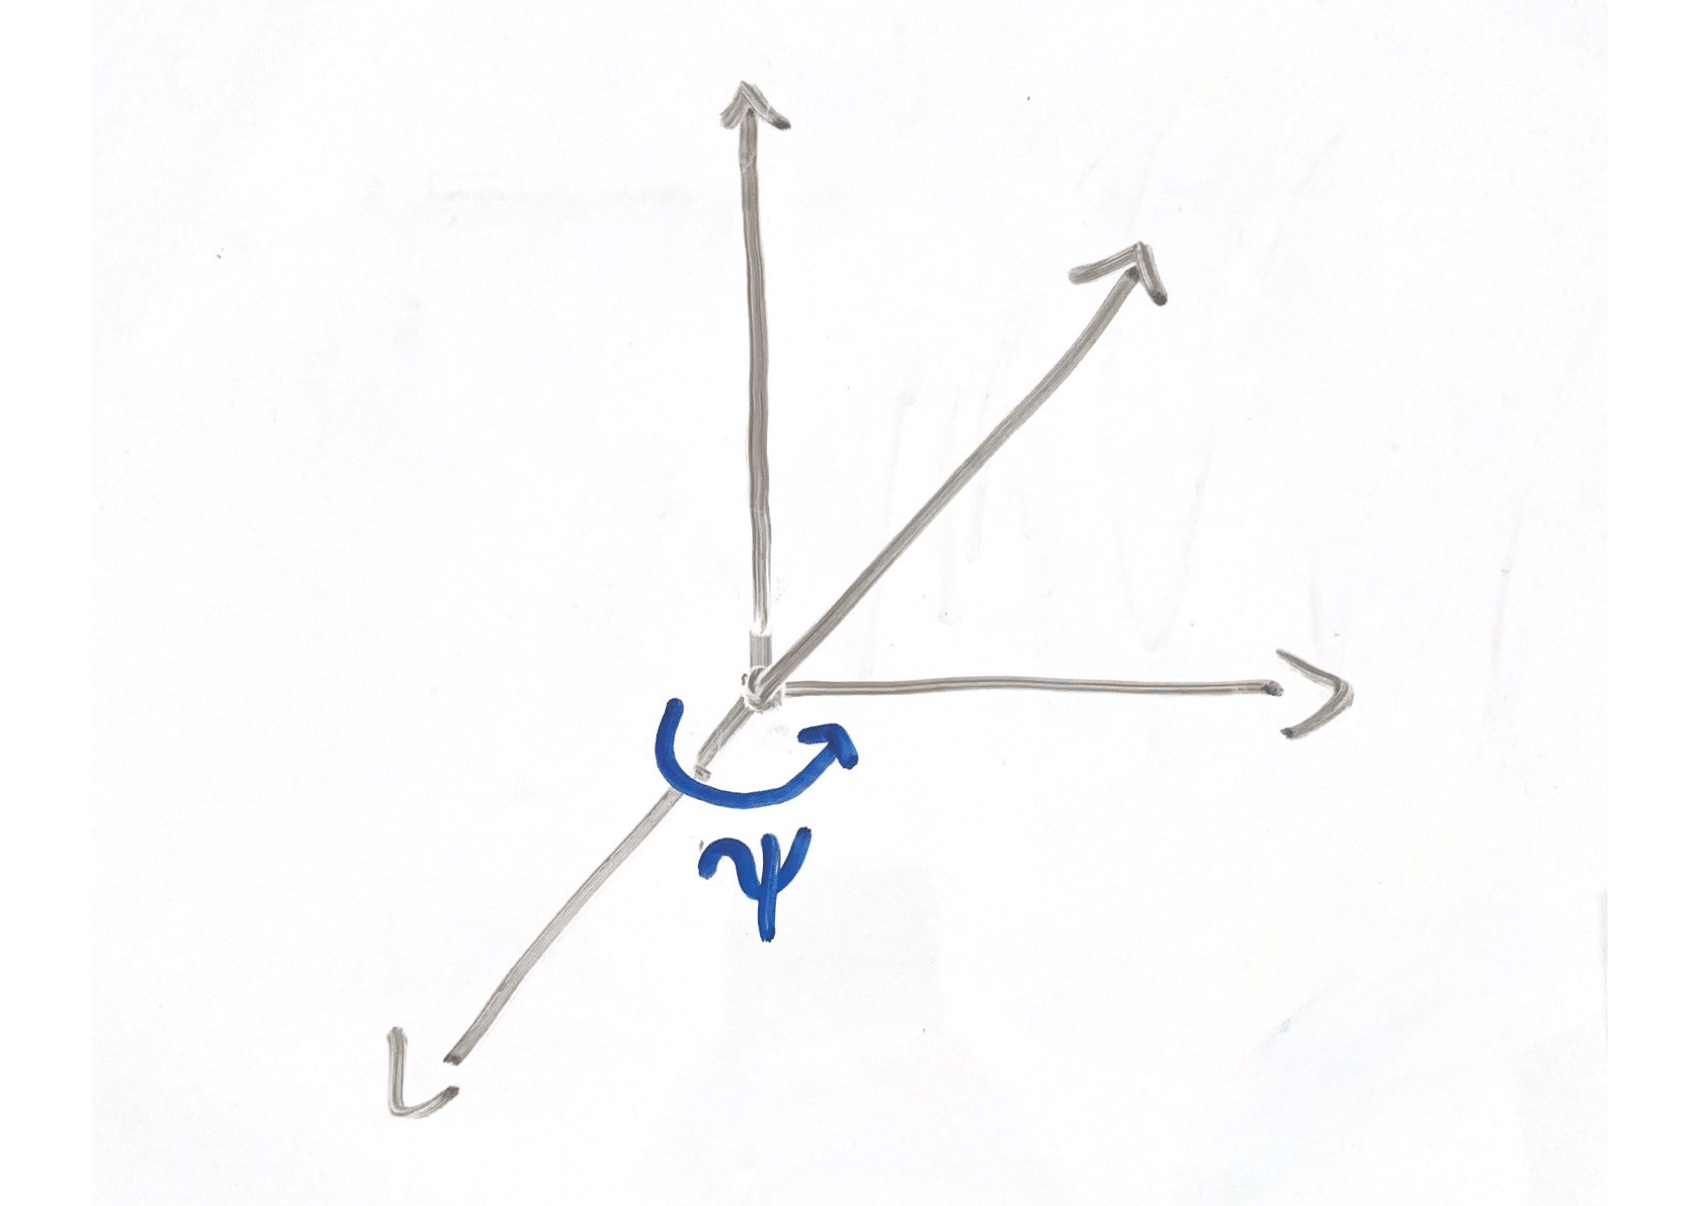
\includegraphics[width=0.2\textwidth]{Rnpsi1.png}
&
		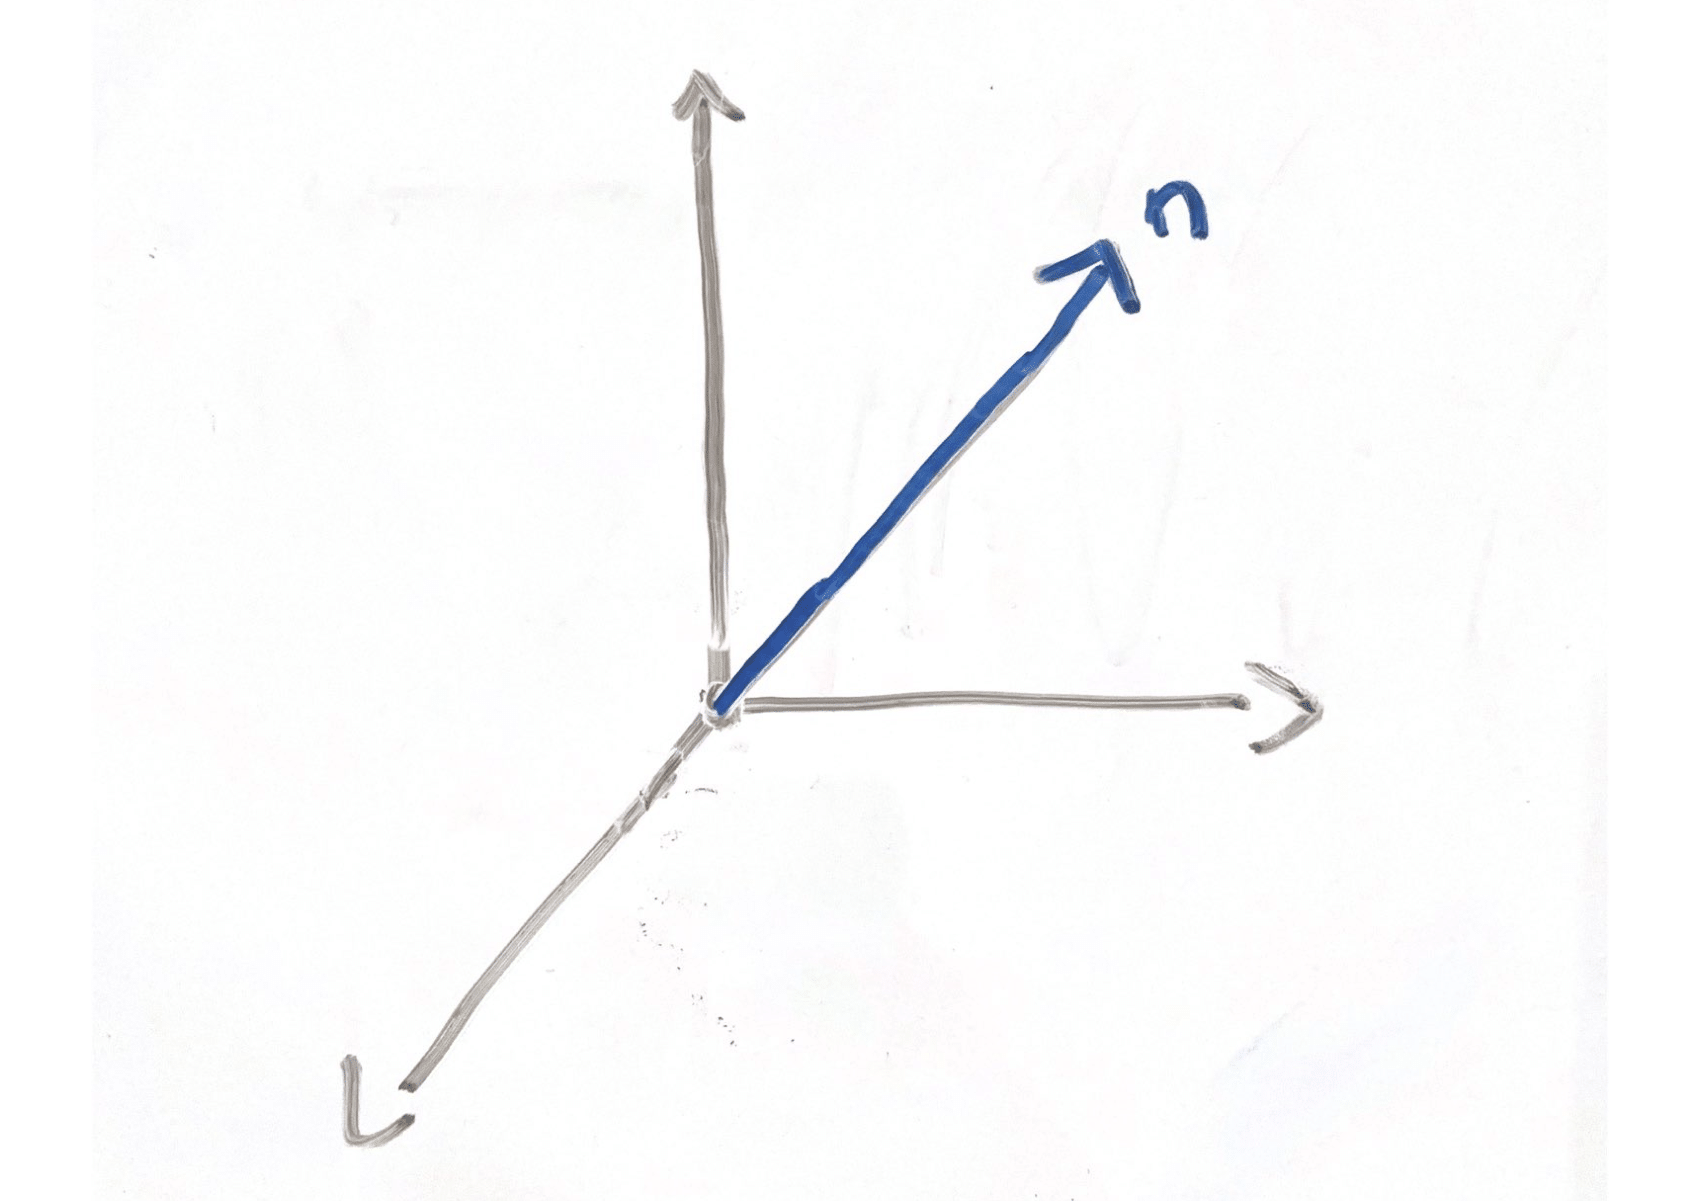
\includegraphics[width=0.2\textwidth]{Rnpsi2.png}
	\end{tabular}
	\caption{Theorem 29: $R_n(\psi)$}
\vfill
\end{figure}
\vfill

\begin{figure}[H]
	\centering

	\begin{tabular}{cccc}
		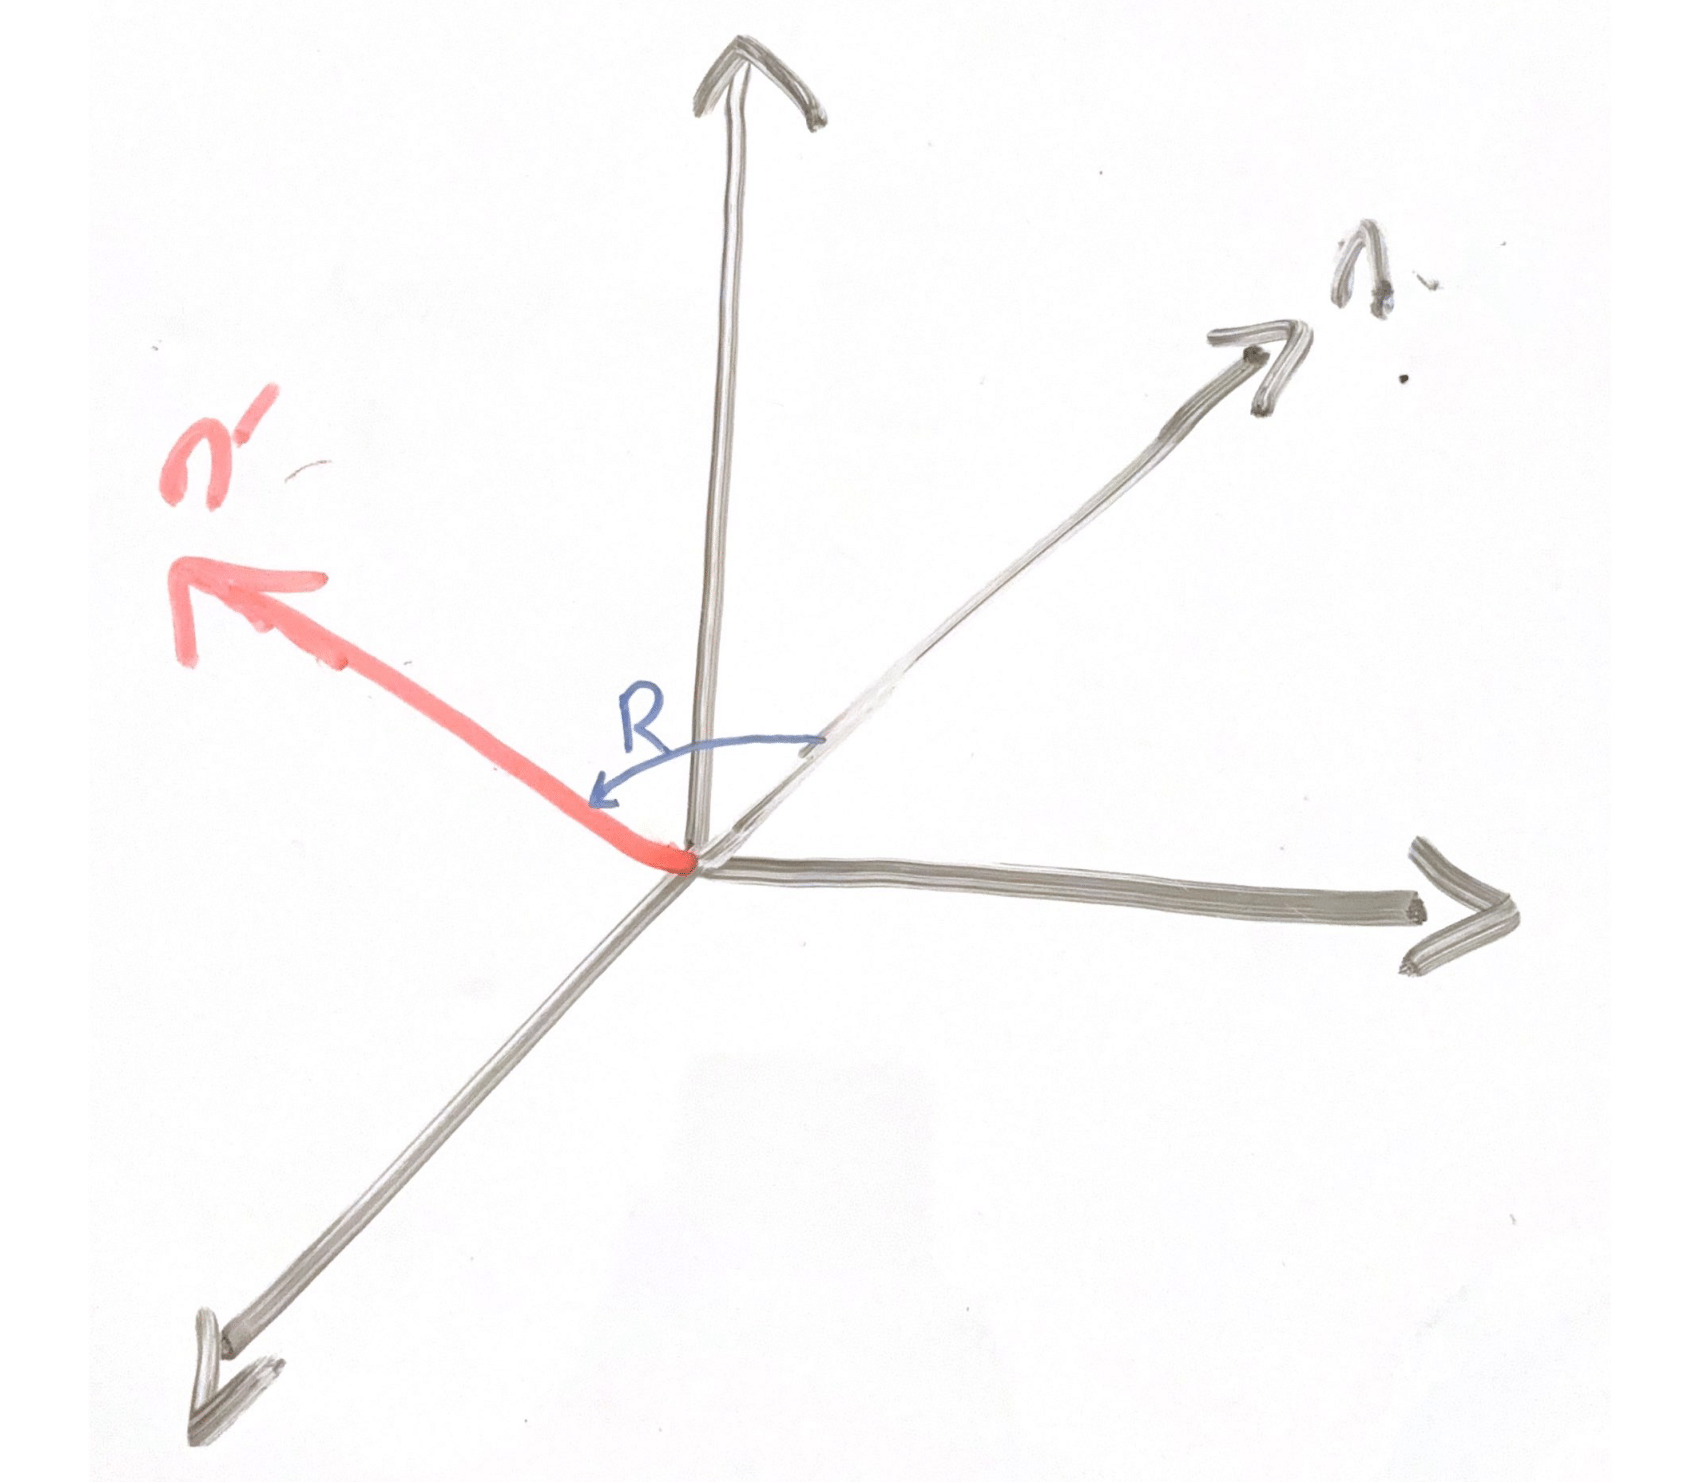
\includegraphics[width=0.2\textwidth]{RRnR1.png}
		&
		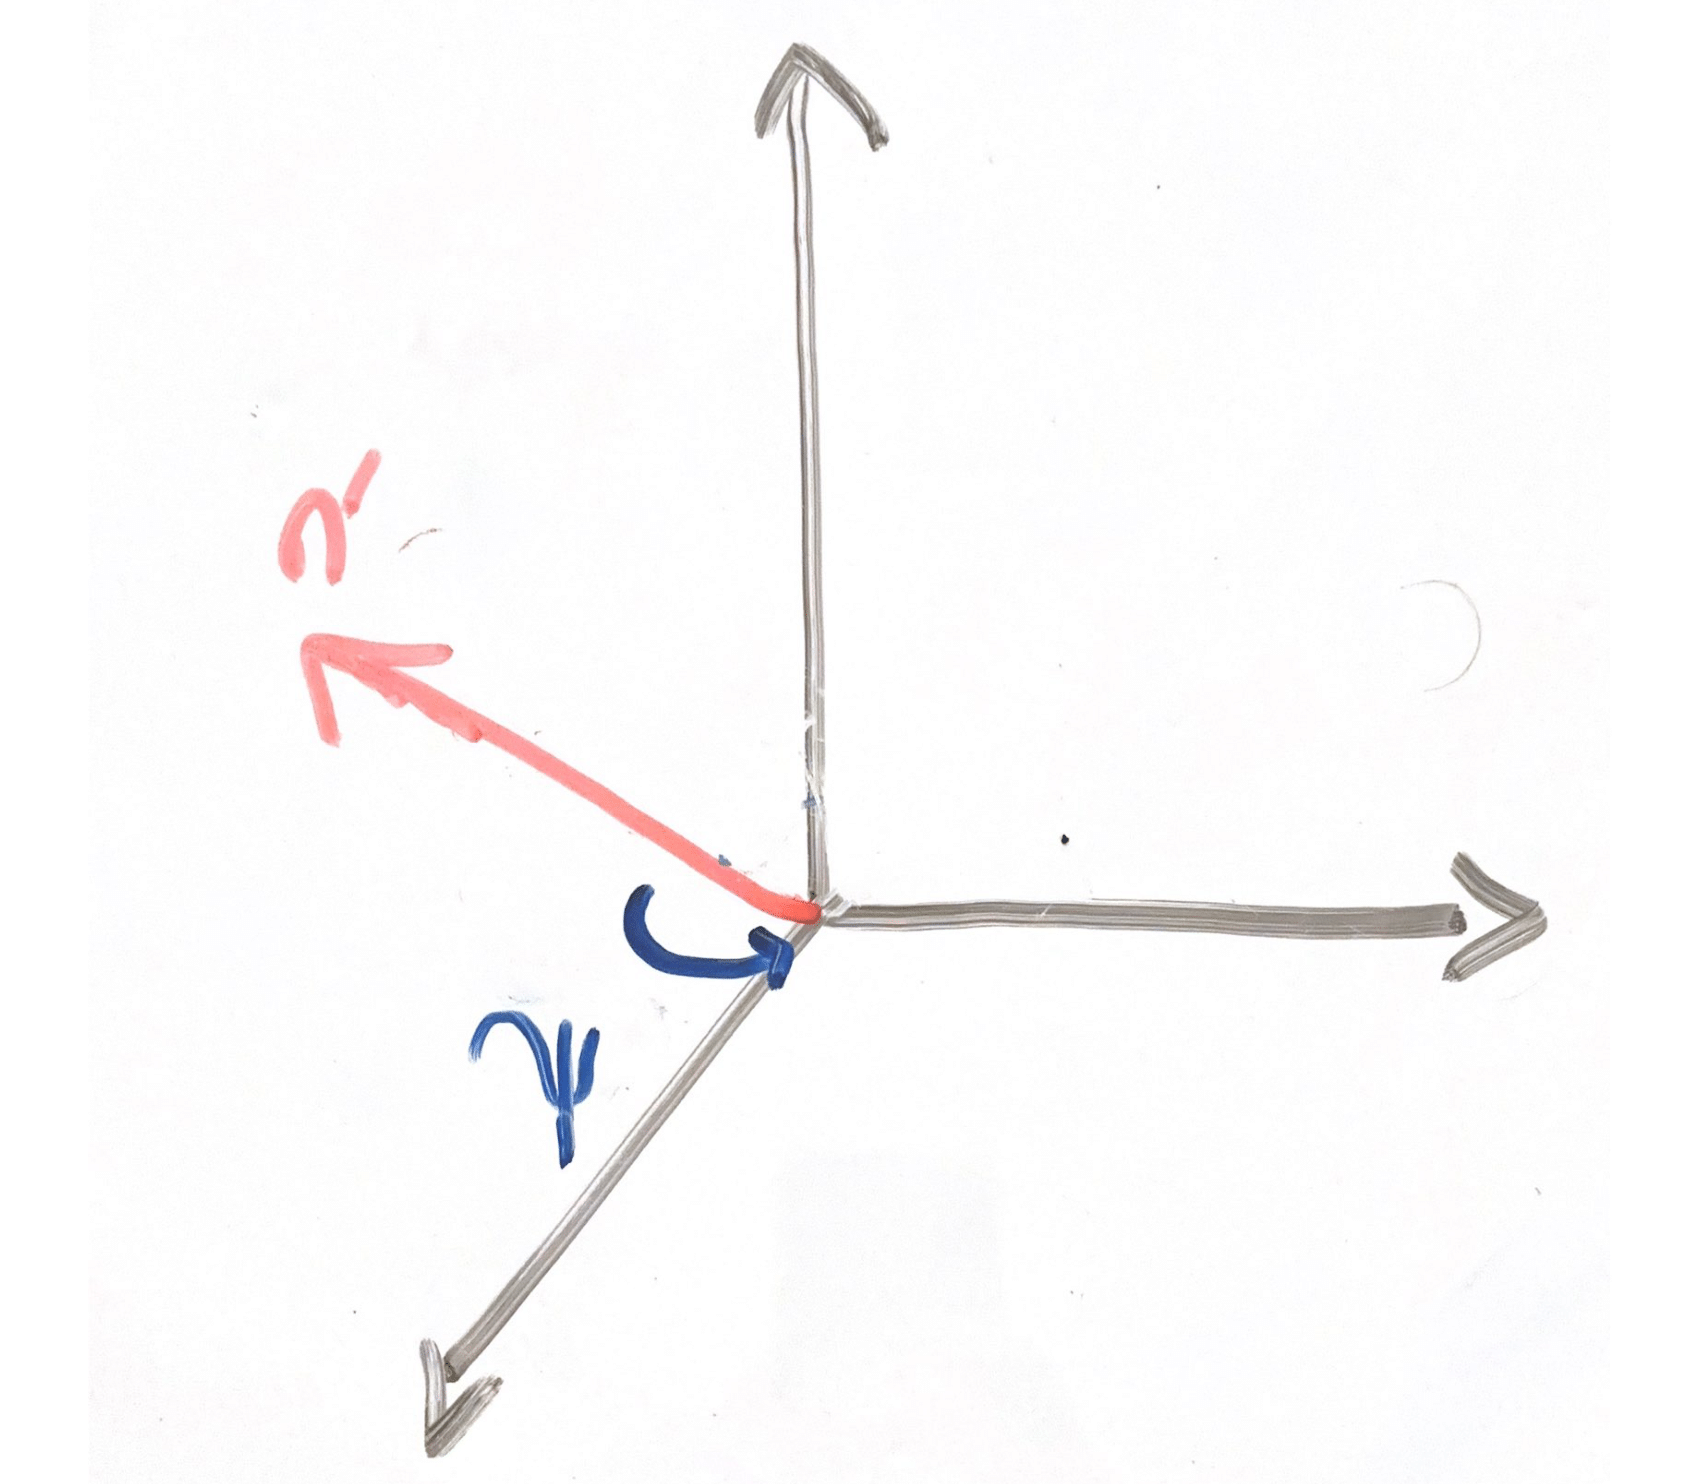
\includegraphics[width=0.2\textwidth]{RRnR2.png}
		&
		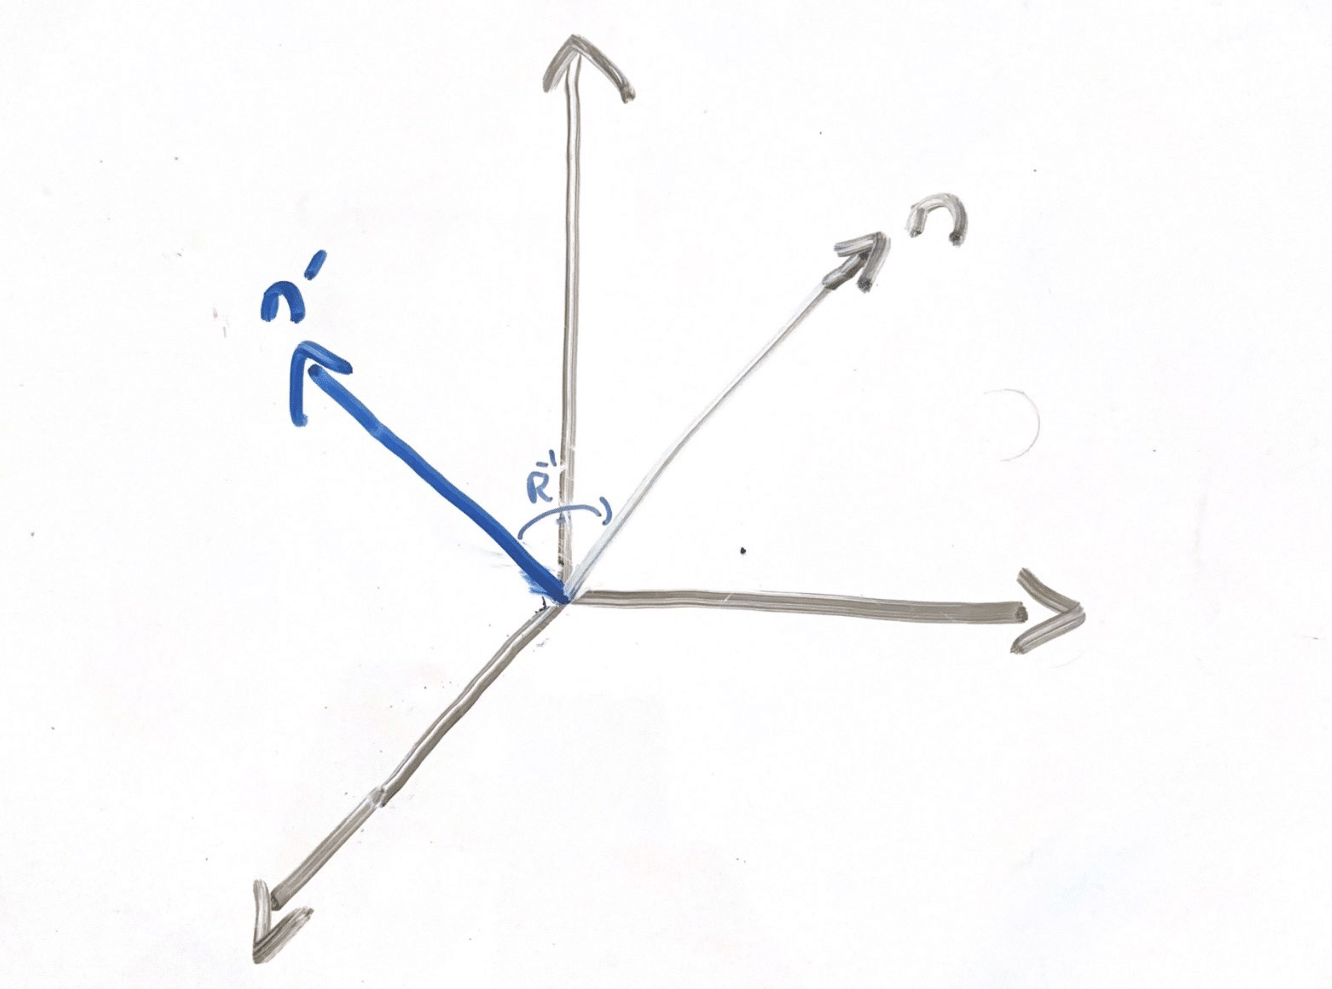
\includegraphics[width=0.2\textwidth]{RRnR3.png}
		&
		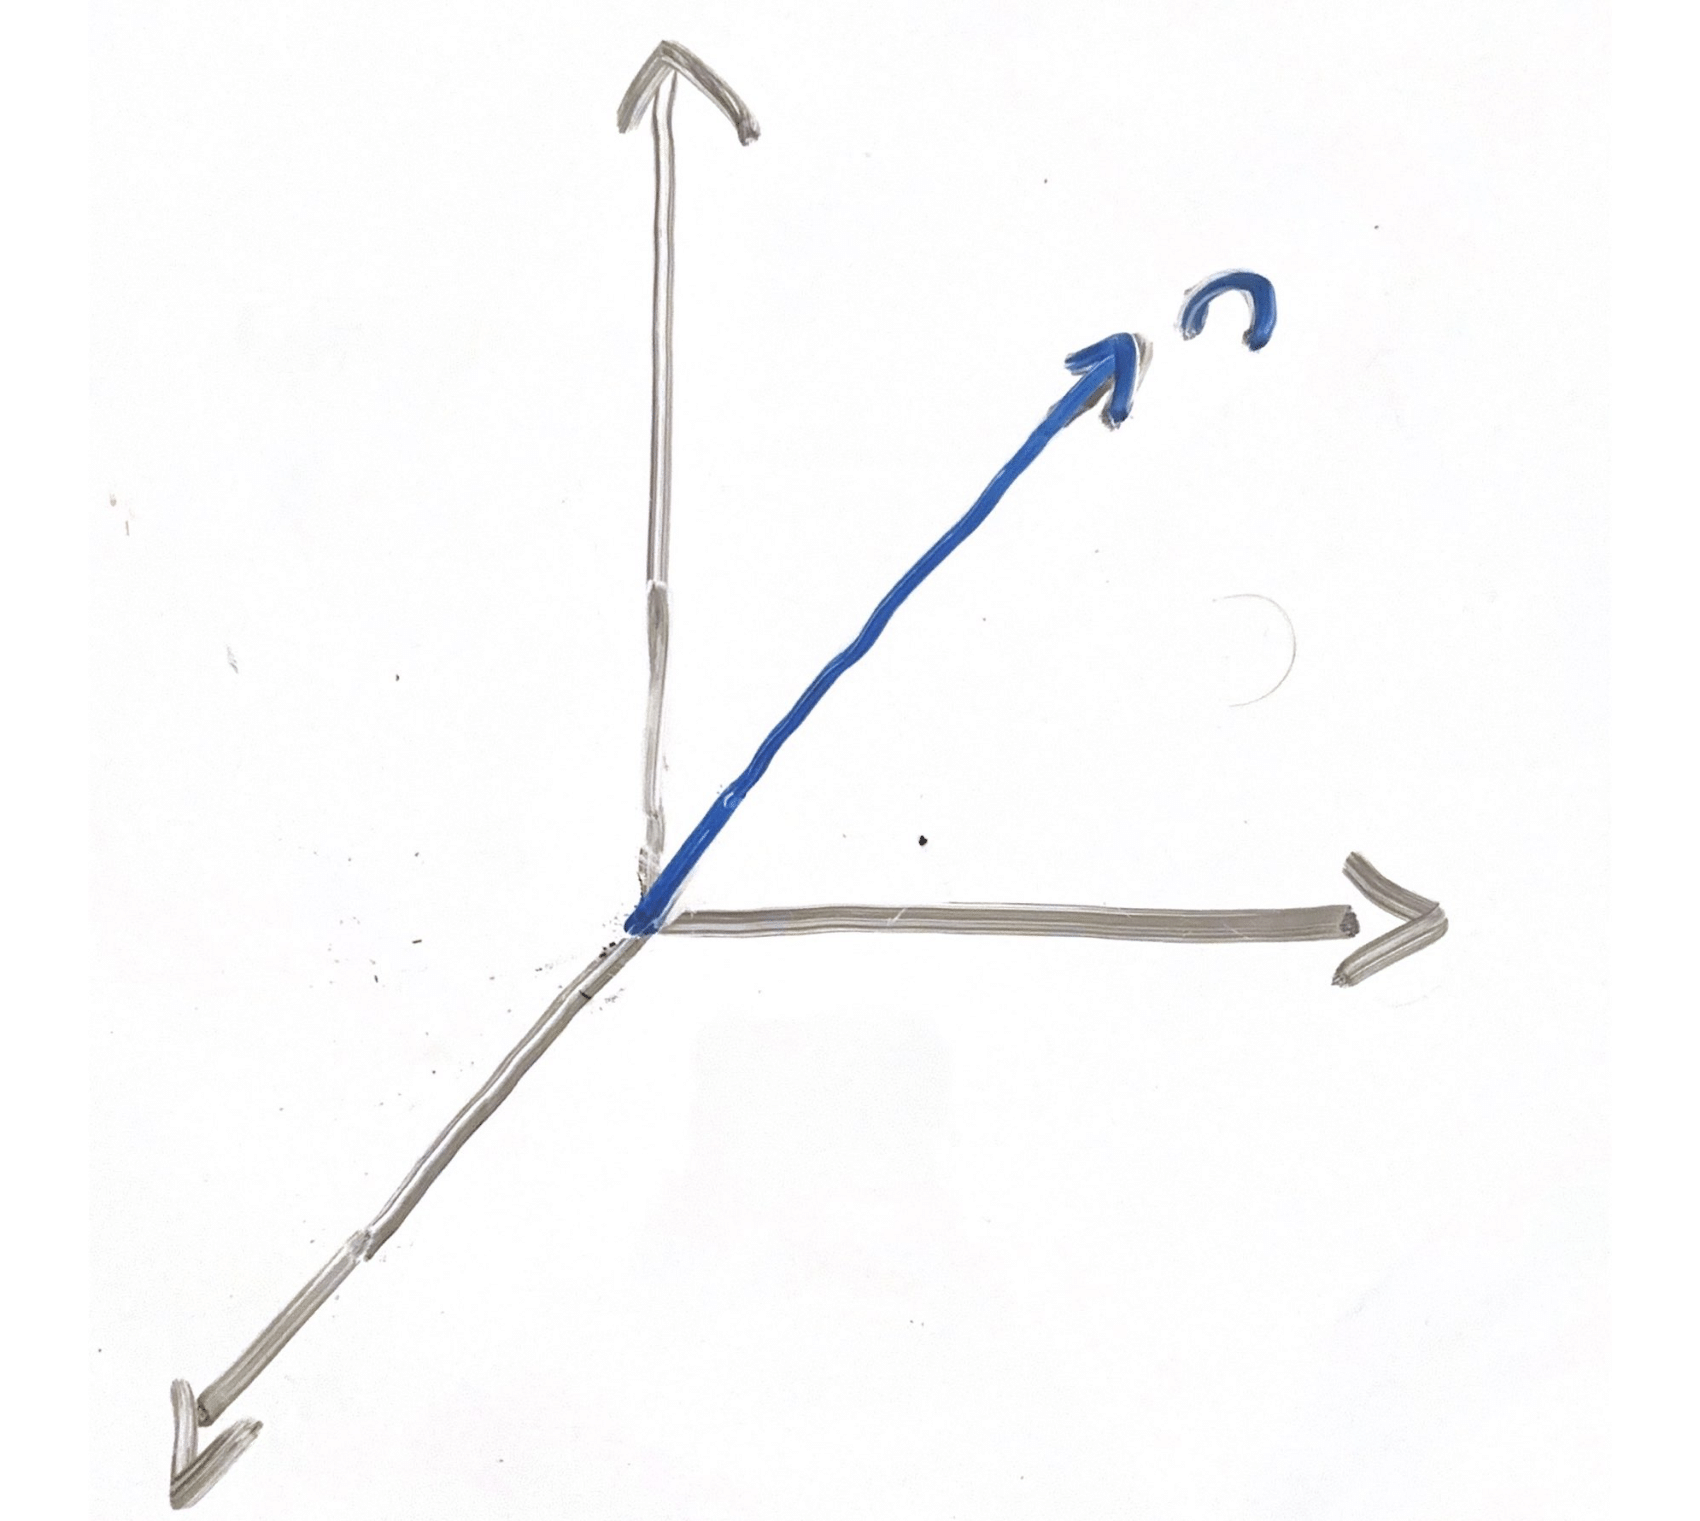
\includegraphics[width=0.2\textwidth]{RRnR4.png}

	\end{tabular}
	\caption{Theorem 29: $R^{-1}R_{n'}(\psi)R$}
\end{figure}
\vfill
\end{frame}

\begin{frame}
\vfill
A direct consecuence of this is 
\vfill
\begin{theorem}
	All rotations (about any axis) by a fixed angle $\psi$ share a conjugacy class (denoted $C_\psi$).
\end{theorem}
\vfill
We can now use our first method of classifying rotations in $SO(3)$ to help build a new way to classify them
\end{frame}
%
%
\begin{frame}
\vfill
Method $2$: Euler Angles
\vfill
\begin{definition}
	Let $(x,y,z)$ be the fixed frame and let $(x',y',z')$ be any rotated frame. Then this rotation's \textbf{Euler Angles} decompose the rotation in the following way:
$$R(\alpha,\beta,\gamma) \coloneq R_{z'}(\gamma)R_n(\beta)R_z(\alpha)$$
where $n$ points in the direction defined by the intersection of the $xy$ and $x'y'$ planes (or equivalently, the $z\times z'$ direction). Note: we use the subscript $z$ and $z'$ as a shorthand to mean the $z$-axis and $z'$-axis.
\end{definition}
\vfill
We can see this idetification in the following successive images:
\end{frame}

\begin{frame}
\vfill
\begin{columns}[T]
\begin{column}{0.3\textwidth}
	\begin{figure}[H]
		\centering
		\tdplotsetmaincoords{60}{200}
		\tdplotsetrotatedcoords{60}{45}{225}
		\begin{tikzpicture}
				[scale=1,
					tdplot_main_coords,
					axis/.style={->,black,thin},
					vector/.style={-stealth,black,very thick}]
			\draw[axis,color=gray] (0,0,0) -- (1,0,0) node[anchor=south]{$x$};
			\draw[axis,color=gray] (0,0,0) -- (0,1,0) node[anchor=west]{$y$};
			\draw[axis] (0,0,0) -- (0,0,1) node[anchor=east]{$z$};
			\draw[axis,color=blue] (0,0,0) -- (-0.707106781186548,0.707106781186548,0) node[anchor=south west]{$z'$}; 
			\tdplotcrossprod(-0.707106781186548,0.707106781186548,0)(0,0,1);
			\draw[axis,color=red] (0,0,0)--(\tdplotresx,\tdplotresy,\tdplotresz) node[anchor=south]{$n$};
			\tdplotdrawarc[->]{(0,0,0)}{1.2}{0}{315}{anchor=north}{$\alpha$};
		\end{tikzpicture}
		\caption{Euler Angles: Rotating Fixed Frame about $z$-axis by $\alpha$}
	\end{figure}
\begin{figure}[H]
	\centering
	\tdplotsetmaincoords{60}{200}
	\tdplotsetrotatedcoords{45}{90}{90}
	
	\begin{tikzpicture}
			[scale=1,
				tdplot_main_coords,
				axis/.style={->,black,thin},
				vector/.style={-stealth,black,very thick}]
		\draw[axis,color=lightgray] (0,0,0) -- (1,0,0) node[anchor=north]{$x$};
		\draw[axis,color=black] (0,0,0) -- (-0.5,-0.5,0.70711) node[anchor=south]{$x'$};
		\draw[axis,color=lightgray] (0,0,0) -- (0,1,0) node[anchor=west]{$y$};
		\draw[axis,color=wildwatermelon] (0,0,0) -- (0.5,0.5,0.70711) node[anchor=south east]{$y'$};
		\draw[axis,color=lightgray] (0,0,0) -- (0,0,1) node[anchor=east]{$z$};
		\draw[axis,color=cobalt] (0,0,0) -- (-0.707106781186548,0.707106781186548,0) node[anchor=east]{$z'$}; 
		\tdplotcrossprod(-0.707106781186548,0.707106781186548,0)(0,0,1);
	
	
		\tdplotdrawarc[->,color=lightgray]{(0,0,0)}{1.2}{0}{315}{anchor=north west}{$\alpha$};
		\tdplotdrawarc[<-,tdplot_rotated_coords,color=classicrose]{(0,0,0)}{1.2}{0}{90}{anchor=north west}{$\beta$};
		\tdplotsetrotatedcoords{135}{90}{180}
		\tdplotdrawarc[->,tdplot_rotated_coords,color=columbiablue]{(0,0,0)}{1.2}{0}{315}{anchor=south}{$\gamma$};
	
	\end{tikzpicture}
	\caption{Euler Angles: Rotated Frame}
\end{figure}

\end{column}
	
\begin{column}{0.3\textwidth}
	\begin{figure}[H]
		\centering
		\tdplotsetmaincoords{60}{200}
		\tdplotsetrotatedcoords{45}{90}{90}
		\begin{tikzpicture}
				[scale=1,
					tdplot_main_coords,
					axis/.style={->,black,thin},
					vector/.style={-stealth,black,very thick}]
			\draw[axis,color=lightgray] (0,0,0) -- (1,0,0) node[anchor=south]{$x$};
			\draw[axis,color=black] (0,0,0) -- (0.7071,-0.7071,0) node[anchor=north]{$x$};
			\draw[axis,color=lightgray] (0,0,0) -- (0,1,0) node[anchor=west]{$y$};
			\draw[axis,color=black] (0,0,0) -- (0,0,1) node[anchor=east]{$z$};
			\draw[axis,color=blue] (0,0,0) -- (-0.707106781186548,0.707106781186548,0) node[anchor=east]{$z'$};
			\tdplotcrossprod(-0.707106781186548,0.707106781186548,0)(0,0,1);
			\draw[axis,color=wildwatermelon] (0,0,0)--(\tdplotresx,\tdplotresy,\tdplotresz) node[anchor=south]{$y$};
			\tdplotdrawarc[->,color=gray]{(0,0,0)}{1.2}{0}{315}{anchor=south east}{$\alpha$};
			\tdplotdrawarc[<-,tdplot_rotated_coords,color=red]{(0,0,0)}{1.2}{0}{90}{anchor=south west}{$\beta$};
		\end{tikzpicture} 
		\caption{Euler Angles: Rotating Intermediate Frame about new $y$-axis by $\beta$}
	\end{figure}
\begin{figure}[H]
	\centering
	\tdplotsetmaincoords{60}{200}
	\tdplotsetrotatedcoords{45}{90}{90}
	\begin{tikzpicture}
			[scale=1,
				tdplot_main_coords,
				axis/.style={->,black,thin},
				vector/.style={-stealth,black,very thick}]
		\draw[axis,color=lightgray] (0,0,0) -- (1,0,0) node[anchor=north]{$x$};
		\draw[axis,color=black] (0,0,0) -- (-0.5,-0.5,0.70711) node[anchor=south]{$x'$};
		\draw[axis,color=lightgray] (0,0,0) -- (0,1,0) node[anchor=west]{$y$};
		\draw[axis,color=black] (0,0,0) -- (0.5,0.5,0.70711) node[anchor=north east]{$y'$};
		\draw[axis,color=lightgray] (0,0,0) -- (0,0,1) node[anchor=east]{$z$};
		\draw[axis,color=black] (0,0,0) -- (-0.707106781186548,0.707106781186548,0) node[anchor=east]{$z'$}; 
		\draw[axis,color=red] (0,0,0) -- (0.707106781186548,0.707106781186548,0) node[anchor=north]{$n$}; 
	
		\coordinate (p1) at (1.1,1.1,0);
		\coordinate (p2) at (-1.1,1.1,0);
		\coordinate (p3) at (-1.1,-1.1,0);
		\coordinate (p4) at (1.1,-1.1,0);
		\coordinate (p5) at  (1.1,1.1,1);
		\coordinate (p6) at (1.1,1.1,-1);
		\coordinate (p7) at (-1.1,-1.1,-1);
		\coordinate (p8) at (-1.1,-1.1,1);
	
	
	
		\draw[color=lightgray] (p1) -- (p2);
		\draw[color=lightgray] (p2) -- (p3);
		\draw[color=lightgray] (p3) -- (p4);
		\draw[color=lightgray] (p4) -- (p1);
		\draw[color=black] (p5) -- (p6);
		\draw[color=black] (p6) -- (p7);
		\draw[color=black] (p7) -- (p8);
		\draw[color=black] (p8) -- (p5);
		\draw[dashed,color=red,very thin] (1.1,1.1,0)--(-1.1,-1.1,0);
	
	\end{tikzpicture}

	\caption{Euler Angles: Identifying $n$}

\end{figure} 
\end{column}
	
\begin{column}{0.3\textwidth}
	\begin{figure}[H]
		\centering
		\tdplotsetmaincoords{60}{200}
		\tdplotsetrotatedcoords{45}{90}{90}
		\begin{tikzpicture}
				[scale=1,
					tdplot_main_coords,
					axis/.style={->,black,thin},
					vector/.style={-stealth,black,very thick}]
			\draw[axis,color=lightgray] (0,0,0) -- (0.7071,-0.7071,0) node[anchor=north]{$x$};
			\draw[axis,color=black] (0,0,0) -- (0,0,1) node[anchor=south]{$x$};
	
			\draw[axis,color=cobalt] (0,0,0) -- (-0.707106781186548,0.707106781186548,0) node[anchor=west]{$z'$}; %(-sqrt(2)/2,sqrt(2)/2,0)
	
			\tdplotcrossprod(-0.707106781186548,0.707106781186548,0)(0,0,1);
			\draw[axis,color=wildwatermelon] (0,0,0)--(\tdplotresx,\tdplotresy,\tdplotresz) node[anchor=south]{$y$};
	
			\tdplotdrawarc[->,color=lightgray]{(0,0,0)}{1.2}{0}{315}{anchor=south east}{$\alpha$};
			\tdplotdrawarc[<-,tdplot_rotated_coords,color=classicrose]{(0,0,0)}{1.2}{0}{90}{anchor=south west}{$\beta$};
			\tdplotsetrotatedcoords{135}{90}{180}
			\tdplotdrawarc[->,tdplot_rotated_coords,color=cobalt]{(0,0,0)}{1.2}{0}{315}{anchor=south}{$\gamma$};
		\end{tikzpicture}
		\caption{Euler Angles: Rotating Intermediate Frame about new $z$-axis by $\gamma$}
	\end{figure}
\end{column}
\end{columns}
\vfill
\end{frame}
%
%
\begin{frame}
\vfill
These rotations illustrate the following identities
\vfill
\begin{equation}
	\begin{aligned}
		R_{z'}(\gamma) = R_n(\beta)R_z(\gamma)R_n(\beta)^{-1}
	\end{aligned}
\end{equation}
\begin{equation}
	\begin{aligned}
		R_n(\beta) = R_z(\alpha)R_y(\beta)R_z(\alpha)^{-1}
	\end{aligned}
\end{equation}
\vfill
Leading to the conclusion that every rotation in $SO(3)$ is characterized by:
\vfill
\begin{equation}
	\begin{aligned}
		R(\alpha,\beta,\gamma) = R_z(\alpha)R_y(\beta)R_z(\gamma)
	\end{aligned}
\end{equation}
\vfill
\end{frame}



\begin{frame}
\vfill
We can use our knowledge of $\R^3$ to immediately build rotation matrices about the coordinate axes
\vfill
\begin{center}
\begin{tabular}{ccc}
		$R_z(\theta) = \begin{bmatrix}
						\cos(\theta) & -\sin(\theta) & 0 \\
						\sin(\theta) & \cos(\theta) & 0 \\
						0 & 0 & 1 \\
						\end{bmatrix}$
&
		$R_y(\theta) = \begin{bmatrix}
						\cos(\theta) & 0& \sin(\theta) \\
						0 & 1 & 0 \\
						-\sin(\theta) &0& \cos(\theta) \\
						\end{bmatrix}$
\end{tabular}
\end{center} \hspace{2mm}
		$$R_x(\theta) = \begin{bmatrix}
						1 & 0 & 0 \\
						0 & \cos(\theta) & -\sin(\theta) \\
						0 & \sin(\theta) & \cos(\theta) \\
						\end{bmatrix}$$


\end{frame}
%
%
\begin{frame}
\vfill
Putting it all together, a general rotation matrix, $R(\alpha,\beta,\gamma)$,  takes in the following form:
$$\begin{bmatrix}
	\cos(\alpha)\cos(\beta)\cos(\gamma) - \sin(\alpha)\sin(\gamma)& -\cos(\alpha)\cos(\beta)\sin(\gamma) -\sin(\alpha)\cos(\gamma)&  \cos(\alpha)\sin(\beta)\\
	\sin(\alpha)\cos(\beta)\cos(\gamma) + \cos(\alpha)\sin(\gamma)& -\sin(\alpha)\cos(\beta)\sin(\gamma) +\cos(\alpha)\cos(\gamma)  &  \sin(\alpha)\sin(\beta) \\
	-\sin(\beta)\cos(\gamma) & \sin(\beta)\sin(\gamma) & \cos(\beta)\\
	\end{bmatrix}$$
\vfill
\end{frame}


\begin{frame}
\vfill
Now that we have characterized the matrices in this group, we want to search for generators.
\vfill
We can find generators of rotations about a fixed axis in the same way as we did in $SO(2)$.
\vfill
\begin{center}
\begin{tabular}{ccc}
		$		J_x = \begin{bmatrix}
					0 & 0 & 0 \\
					0 & 0 & -i \\
					0 & i & 0
					\end{bmatrix}$
&
		$		J_y = \begin{bmatrix}
					0 & 0 & i \\
					0 & 0 & 0 \\
					-i & 0 & 0
					\end{bmatrix}$
\end{tabular}
		$$J_z = \begin{bmatrix}
					0 & -i & 0 \\
					i & 0 & 0 \\
					0 & 0 & 0
					\end{bmatrix}$$
\end{center}
\end{frame}
%
%
\begin{frame}
\vfill
\begin{theorem}
	 For any arbitrary direction, $n=(n_1,n_2,n_3)\in\R^3$, the generator, $J_n$, can be written in the following way:
$$J_n = n_1J_x + n_2J_y + n_3J_z$$
\end{theorem}
\vfill
As a result, we can write any rotation in the following equivalent ways depending on our convention:
\begin{equation}
	\begin{aligned}
		R_n(\psi) = e^{-i\psi n_1J_x}e^{-i\psi n_2J_y}e^{-i\psi n_3J_z}
	\end{aligned}
\end{equation} 
\begin{equation}
	\begin{aligned}
		R(\alpha,\beta,\gamma) = e^{-i\alpha J_z}e^{-i\beta J_y}e^{-i\gamma J_z}
	\end{aligned}
\end{equation} 
\end{frame}


\begin{frame}
\vfill
In order to find invariant subspaces, we seek eigenvectors of all our generators.
\vfill
\begin{block}{General Strategy}
Find a set of generators that commute, and therefore, have matching eigenvalues and matching eigenvectors.
\end{block}
\vfill
Unfortunately, none of our generators commute.
\vfill
\end{frame}
%
%
\begin{frame}
\vfill
\begin{definition}
	The \textbf{commutator} of two matrices $A$ and $B$ is defined by to be 
$$[A,B]=AB-BA$$
\end{definition}
\vfill
\begin{theorem}
	Let $J_k,J_l \in \{J_x,J_y,J_z\}$. Consider the word $xyz$, and all 6 rearrangements of it (identifying each rearrangement with a permutation in $S_3$). Then 
$$[J_k , J_l] = \begin{cases}
					0 & \text{if }k = l \\
					isign(klm)J_m& \text{else}
					\end{cases}$$
where $m$ is the label of the remaining generator in $\{J_x,J_y,J_z\}$.
\end{theorem}
\vfill
\end{frame}


\begin{frame}
\vfill
\begin{definition}
	A \textbf{Lie Algebra} is a vector space, $\mathfrak{g}$, together with a bilinear operation, [ . , . ] that satisfies the the following identities:
\begin{itemize}
	\item$ [x,x] = 0$  $\forall x\in\mathfrak{g}$
	\item $[x,[y,z]] + [y,[z,x]] + [z[y,x]]= 0 $ $\forall x,y,z\in\mathfrak{g}$
\end{itemize}
\end{definition}
\vfill
$$\mathfrak{so}(3) := \{a_1J_x + a_2J_y + a_3Jz \mid a_1,a_2,a_3\in\C\}$$
\vfill
Does not solve our problem $\hdots$ yet.
\end{frame}
%
%
\begin{frame}
\vfill
	\begin{definition}
		The \textbf{universal enveloping algebra} of a Lie algebra is the largest embedding of Lie algebra into an algebra. 
	\end{definition}
\vfill
This space is constructed as a tensor space with the commutator relations of the Lie algebra quotiented out.
\vfill
\begin{definition}
	A \textbf{Casimir element} of a Lie algebra, $A$, is any element in the center of the universal enveloping algebra of $A$.
\end{definition}
\vfill
\end{frame}

\begin{frame}
\vfill
Our Casimir element is one of physical significane (angular-momentum operator)
$$\mathfrak{J^2} \coloneq (\mathfrak{J}_x \otimes \mathfrak{J}_x) \oplus (\mathfrak{J}_y \otimes \mathfrak{J}_y) \oplus (\mathfrak{J}_z \otimes \mathfrak{J}_z) = \mathfrak{J}_x^2 + \mathfrak{J}_y^2 + \mathfrak{J}_z^2$$
\vfill
Since $\mathfrak{J^2}$ commutes with the generators, so does its image through an irreducible representation.
\vfill
Schur's Theorem: 
\begin{equation}
	\begin{aligned}\phi_{\mathfrak{J^2}} = \lambda I_n 	\end{aligned}
\end{equation} 
\vfill
\end{frame}
%
%
\begin{frame}
\vfill
Choose generators (by convention) $\{\mathfrak{J^2}, \mathfrak{J}_z\}$
\vfill
Define raising and lowering generators:
\begin{equation}
	\begin{aligned}
		\mathfrak{J}_\pm = \mathfrak{J}_x \pm i\mathfrak{J}_y
	\end{aligned}
\end{equation} 
\vfill
New commutator relationships:
\begin{equation}
	\begin{aligned}
		[\mathfrak{J}_z,\mathfrak{J}_+] = \mathfrak{J}_+
	\end{aligned}
\end{equation} 
\begin{equation}
	\begin{aligned}
		[\mathfrak{J}_z,\mathfrak{J}_-] = -\mathfrak{J}_-
	\end{aligned}
\end{equation} 
\begin{equation}
	\begin{aligned}
		[\mathfrak{J}_+,\mathfrak{J}_-] = 2\mathfrak{J}_z
	\end{aligned}
\end{equation} 
\begin{equation}
	\begin{aligned}
		\mathfrak{J}^2 = (\mathfrak{J}_z)^2  -\mathfrak{J}_z +\mathfrak{J}_+\mathfrak{J}_- = (\mathfrak{J}_z)^2 +\mathfrak{J}_z+ \mathfrak{J}_-\mathfrak{J}_+
	\end{aligned}
\end{equation} 
\end{frame}

\begin{frame}
\vfill 
For any eigenvector $v_m$ of $\phi_{\mathfrak{J}_z}$, corresponging to eigenvalue $m$.
\begin{equation}
	\begin{aligned}
		\phi_{\mathfrak{J}_z\mathfrak{J}_+}(v_m) = (m + 1)\phi_{\mathfrak{J}_+}(v_m)
	\end{aligned}
\end{equation} 
\begin{equation}
	\begin{aligned}
		\phi_{\mathfrak{J}_z\mathfrak{J}_-}(v_m) = (m -1)\phi_{\mathfrak{J}_-}(v_m)
	\end{aligned}
\end{equation} 
\vfill
We can construct an eigenbasis of our vectorspace by repeated applications of the raising and lowering generators.
\vfill
This process will eventually terminate for finite degree representation.
\vfill
If $k$ is the last nonzero power of $\phi_{\mathfrak{J}_+}$ to $v_0$, and $s$ is the eigenvalue of $\phi_{\mathfrak{J}_+}v_{k-1}$ to the map $\phi_{\mathfrak{J}_z}$, then
\begin{equation}
	\begin{aligned}
		\phi_{\mathfrak{J^2}}\phi_{\mathfrak{J}_+}^k(v_{k-1})= s(s + 1) \phi_{J_+}^kv_{k-1}
	\end{aligned}
\end{equation}
\vfill
\end{frame}
%
%
\begin{frame}
\vfill
\begin{theorem}
	The irreducible representations of the $A_{\mathfrak{so}(3)}$ are characterized by eigenvalues that take on positive integer and positive half-integers. If $\lambda$ is one such eigenvalue, then we can construct our eigenvectors, $\{v_m\}_{m=-\lambda}^\lambda$, corresponding to $\phi_{\mathfrak{J}_z}$ with eigenvalue $m$, using the raising or lowering operators. This gives us a degree $2s +1$ representation characterized by the following relationships:
$$\phi_{\mathfrak{J}^2}(v_m) = s(s+1)v_m$$
$$\phi_{\mathfrak{J}_z}(v_m) =  mv_m$$ 
$$v_{m+1} =  \frac{1}{\sqrt{\lambda(\lambda+1) - m(m\pm 1)}}\phi_{\mathfrak{J}_\pm}(v_m)$$
\end{theorem}
\vfill
\begin{equation}
\begin{aligned}
	\phi_j(R(\alpha,\beta,\gamma)) &= e^{-i\alpha\phi_{\mathfrak{J}_z}}e^{-i\beta\phi_{\mathfrak{J}_y}}e^{-i\gamma\phi_{\mathfrak{J}_z}}	
\end{aligned}
\end{equation}
\vfill
\end{frame}

\section{Euclidean Groups}
\begin{frame}
\sectionpage
\end{frame}
%
%
\begin{frame}
\vfill
\begin{definition}
	The $n$-dimensional \textbf{Euclidean Group, $E_n$,} is the group of all continuous, isometric, linear transformations on $\R^n$.
\end{definition}
\vfill
For any transformation of this kind, all vectors, $x\in\R^n$, get mapped to $x'\in\R^n$ in the following way 
$$x' = Rx + b$$
for some fixed $R\in SO(n)$ and $b\in\R^n$.
\vfill
If we focus on $E_2$, we can construct an invertible matrix to represent each transformation

\begin{equation}
\begin{aligned}\begin{bmatrix}x'_1\\x'_2 \\ 1\end{bmatrix} = \begin{bmatrix}
			\cos(\theta) & -\sin(\theta) & b_1\\
			\sin(\theta) & \cos(\theta) & b_2 \\
			0&0&1
		\end{bmatrix} \begin{bmatrix}x_1\\x_2\\1\end{bmatrix}\end{aligned}
\end{equation}

\end{frame}

\begin{frame}
\vfill
We can derive the generators of $E_2$ in the same way as we did for $SO(2)$ and $SO(3)$.
\vfill
Our rotational generator is the same as in $SO(2)$
\begin{equation}
\begin{aligned}
J=\begin{bmatrix}
			0 & -i & 0\\
			i & 0 & 0 \\
			0 & 0 & 0
		\end{bmatrix}
\end{aligned}
\end{equation}
\vfill
Further, we can use the same process to derive the generators for translations in two directions.\vfill
\end{frame}


%
%
\begin{frame}
If we denote $T_n$ to be the group of translations in $n$-dimensions.
\vfill
Starting with $T_1$, we let $T_b\in T_1$ where $b\in \R$
\begin{equation}
\begin{aligned}
T_{dx} = I -idxP
\end{aligned}
\end{equation}
where $P$ is our generator.
\vfill
We construct our system of equations:
\begin{equation}\begin{aligned}T_{x+dx} = T_x + dx \frac{d}{dx}T_x\end{aligned}\end{equation}
\begin{equation}\begin{aligned}T_{x+dx} = T_{dx}T_x\end{aligned}\end{equation}
\vfill
\end{frame}
%%
\begin{frame}
\vfill
We conclude with 
\begin{equation}\begin{aligned}T(x) = e^{-iPx}\end{aligned}\end{equation}
\vfill
As we generalize to $E_2$,
\begin{equation}\begin{aligned}P_x = \begin{bmatrix}
			0 & 0 & i\\
			0 & 0 & 0 \\
			0 & 0 & 0
		\end{bmatrix}, \hspace{3mm}P_y = \begin{bmatrix}
			0 & 0 & 0\\
			0 & 0 & i \\
			0 & 0 & 0
		\end{bmatrix}\end{aligned}\end{equation}
\vfill
and therefore for any $b\in\R^2$, 
\begin{equation}\begin{aligned}T_b = e^{-ib_1P_x}e^{-ib_2P_y}\end{aligned}\end{equation}
\end{frame}
%
%
\begin{frame}
\vfill
Some useful properties of $E_2$ include
\vfill
\begin{theorem}
	For any $\theta$,$b$
	$$R(\theta)T_bR(\theta)^{-1} = T_{R(\theta)b}$$
\end{theorem}
\vfill
\begin{theorem}
	For any $g(\theta,b)\in E_2$, there is a natural decomposition of the transformation into a pure rotation times a pure translation.
$$g(\theta,b) = g(0,b)g(\theta,0)$$
\end{theorem}
\vfill
\end{frame}


\begin{frame}
When discussing the search for irreducible representations, we follow the same path.
\vfill
Our commutator relationships:
\begin{equation}
\begin{aligned}
	[P_x,P_y] = 0
\end{aligned}
\end{equation}
\begin{equation}
\begin{aligned}
	[J,P_x] = iP_y
\end{aligned}
\end{equation}
\begin{equation}
\begin{aligned}
	[J,P_y] = -iP_x
\end{aligned}
\end{equation}
\vfill
Our raising and lowering generators:
\begin{equation}
\begin{aligned}
	P_\pm \coloneq P_x \pm iP_y
\end{aligned}
\end{equation}
\vfill
And journeying into the universal enveloping algebra, the Casimir element:
\begin{equation}
\begin{aligned}
	\mathfrak{P}^2 = (\mathfrak{P}_x)^2 + (\mathfrak{P}_y)^2 = \mathfrak{P}_+\mathfrak{P}_- = \mathfrak{P}_-\mathfrak{P}_+
\end{aligned}
\end{equation}
\vfill
\end{frame}
%
%
\begin{frame}
\vfill
If we let $\psi$ be our irreducible representation of our universal enveloping algebra,
\begin{equation}
\begin{aligned}
	 \psi(\mathfrak{P}^2)v_m = pv_m,\hspace{3mm} p>0
\end{aligned}
\end{equation}
\begin{equation}
\begin{aligned}
	 \psi(\mathfrak{J})v_m = mv_m, \hspace{3mm} m\in\Z
\end{aligned}
\end{equation}
\vfill 
Unfortunately, there is no termination in the construction of our basis, so we must resort to characterizing our representations by discussing their matrix elements.
\vfill
\end{frame}


\begin{frame}
\vfill
\begin{theorem}
	The faithful, unitary, irreducible representations of $E_2$ are characterized by the following equation defined in terms of matrix elements. If $\psi_p$ is a representation corresponding to a $p>0$, then $[\psi_p(g)]_{mm'}$ corresponds to the matrix element specified by the choice of $v_m$, $v_{m'}$, and $g$. The representations, $\psi_p$ have the following form:
$$[\psi_p(g(\theta,b))]_{mm'} = e^{i(m-m')\phi}J_{m-m'}(pr)e^{-im\theta}$$
where $r$ and $\phi$ are the polar coordinates for the vector $b$.
\end{theorem}
\vfill
\end{frame}
%
%
\begin{frame}
\vfill
Regarding $E_3$, we can decompose any transformation as 
\begin{equation}
\begin{aligned}
	x' =
	\begin{bmatrix}
		\underset{3\times 3}{R(\alpha,\beta,\gamma)} & \underset{3\times 1}{b}\\
		\underset{1\times 3}{0} & 1
	\end{bmatrix} x
\end{aligned}
\end{equation}
\vfill
Our generators $\{J_x,J_y,J_z,P_x,P_y,P_z\}$ as defined in $SO(3)$ and implicitly $T_3$ satisfy
\begin{equation}
\begin{aligned}
	T_b = e^{-ib_1P_x}e^{-ib_2P_y}e^{-ib_3P_z}
\end{aligned}
\end{equation}
\begin{equation}
\begin{aligned}
	R(\alpha,\beta,\gamma) = e^{-i\alpha J_z}e^{-i\beta J_y}e^{-i\gamma J_z}
\end{aligned}
\end{equation}	
\vfill
\end{frame}

\begin{frame}
\vfill
Our commutator relations:
\vfill
\begin{equation}
\begin{aligned}
	[P_k,P_l] = 0 \hspace{3mm} \forall k,l\in \{x,y,z\}
\end{aligned}
\end{equation}
\begin{equation}
\begin{aligned}
	[J_k,J_l] = \begin{cases}
					0 & \text{if } k = l\\
					isign(klm)J_m & else
					\end{cases}
\end{aligned}
\end{equation}
where $m$ is the remaining label for the unused generator in the commutator.
\begin{equation}
\begin{aligned}
	[P_k,J_l] = \begin{cases}
					0 & \text{if } k = l\\
					isign(klm)P_m & else \end{cases}
\end{aligned}
\end{equation}
\vfill
\end{frame}
%
%
\begin{frame}
\vfill
Useful Identities:
\vfill
\begin{theorem}
For any $R\in SO(3)$, $T_b\in T_3$,
$$RT_bR^{-1} = T_{b'}$$
\end{theorem}
\vfill
\begin{theorem}
For any $g\in E_3$, $$g = R(\alpha,\beta,\gamma)T_b\text{ for some } b\in\R^3, R\in SO(3)$$
\end{theorem}
\vfill
\end{frame}

\begin{frame}
\vfill
In the universal enveloping algebra, we actually have two Casimir operators:
\begin{equation}\begin{aligned}\mathfrak{P^2}\coloneq (\mathfrak{P}_x)^2 + (\mathfrak{P}_y)^2 + (\mathfrak{P}_z)^2\end{aligned}\end{equation} \begin{equation}\begin{aligned}\mathfrak{J}* \mathfrak{P} \coloneq \mathfrak{J}_x\mathfrak{P}_x +\mathfrak{J}_y\mathfrak{P}_y + \mathfrak{J}_z\mathfrak{P}_z\end{aligned}\end{equation}
\vfill
Constructing our irreducible representations as we have done previously will result in a trivial case. Eigenvalues are no longer going to help us.
\vfill
\begin{definition}
	Let $G$ be a group, $N$ be a normal subgroup, $\phi$ be a representation of $G$, and $V$ be the underlying vector space of the representation. Then for any $v\in V$, the \textbf{little group} of $v$ is the subgroup of $G/N$ who's image under $\phi$ leave $v$ invariant.
\end{definition}
\vfill
\end{frame}
%
%
\begin{frame}
\vfill
\begin{block}{Strategy}
\begin{itemize}
	\item Find a nice normal subgroup, quotient out ($T_3$)
	\item Pick a nonzero starting vector
	\item Find representations of the little group of said vector
	\item Transform vector to recover remaining vectors, repeat process for general representation
	\item We are left with the smallest invariant subspace (generated by one vector)
\end{itemize}
\end{block}
\vfill
Let our starting choice in this case be $p_0 = \mu_ze_z$.
\end{frame}


\begin{frame}
\vfill
The only rotations that leave $p_0$ unaffected are about the $z-axis$. The little group of $p_0$ is isomorphic to $SO(2)$.
\vfill
The irreducible representations of $SO(2)$ are indexed by $\lambda\in\Z$.
\begin{equation}
\begin{aligned}\psi_{\mathfrak{J}_z}p_0 = \lambda p_0
\end{aligned}\end{equation}
\vfill
Further, we have the following relationships between our other generators:
\begin{equation}
\begin{aligned}\psi_{\mathfrak{P}_x}p_0 = \psi_{\mathfrak{P}_y}p_0 = 0
\end{aligned}
\end{equation}
\begin{equation}
\begin{aligned}
\psi_{\mathfrak{P}_z}p_0 = \mu_z p_0
\end{aligned}
\end{equation}
\begin{equation}
\begin{aligned}
	\psi_{\mathfrak{JP}}p_0 = \mu_z\lambda p_0
\end{aligned}
\end{equation}
\begin{equation}
\begin{aligned}
	\psi_{\mathfrak{P}^2}p_0 = \mu_z^2p_0
\end{aligned}
\end{equation}
\vfill
\end{frame}
%
%
\begin{frame}
\vfill
We then conclude that
\vfill
\begin{equation}
\begin{aligned}
	\psi(R_z(\theta)) p_0 = e^{-i\lambda\theta}p_0
\end{aligned}
\end{equation}
\begin{equation}
\begin{aligned}
	\psi(T_b) p_0 = e^{-i\mu b_3}p_0
\end{aligned}
\end{equation}
\vfill
Now that we know the value our representation can take on this vector, let us rotate this vector $p_0$ by the rotation $R(\alpha,\beta,0)$ to $p$. 
\vfill
We can repeat this process, finding the eigenvalues corresponding to our generators.
\end{frame}

\begin{frame}
\vfill
\begin{theorem}
The irreducible unitary representations are characterized by $\lambda\in\Z$ and the following equations:
\begin{equation}
\begin{aligned}
	\psi(T_b) p = e^{-ib_1\mu_x}e^{-ib_2\mu_y}e^{-ib_3\mu_z}p
\end{aligned}
\end{equation}
\begin{equation}
\begin{aligned}
	\psi(R(\alpha,\beta,\gamma)) p = e^{-i\lambda\xi}p'
\end{aligned}
\end{equation}
where $p' = R(\alpha,\beta,\gamma)p$, the cylindrical angles of $p'$ are $\theta'$ and $\phi'$, and $\xi$ is the angle ascertained from the equation $R(0,0,\xi)=R(\phi',\theta',0)^{-1}R(\alpha,\beta,\gamma) R(\phi,\theta,0)$. 
\end{theorem}
\vfill
\end{frame}
%
\section{Lorentz and Poincar\'e Groups}
\begin{frame}
\sectionpage
\end{frame}

\begin{frame}
\vfill
The coming spaces we will study are non-Euclidean
\vfill
\begin{definition}
	An \textbf{event} is an ordered triple together with an additional parameter, meant to represent time. An event is conventionally indexed by the integers $\mu = 0,1,2,3$. Referring to an event as $x$ references the event a four (component) vector, and specifying $x^{\mu=0}$ gives us $ct$ where $c$ is the speed of light and $t$ is a time. 
\end{definition}
\vfill
\begin{definition}
	The \textbf{length} of an event is defined by the following equation:
$$\mid x\mid^2 \coloneq (x^1)^2+(x^2)^2+(x^3)^2 - (x^0)^2 = (x^1)^2+(x^2)^2+(x^3)^2 - c^2t^2$$
\end{definition}
\end{frame}
%
%
\begin{frame}
\vfill
$$\begin{array}{c@{\hskip 1cm}c}

	\underset{\text{Euclidean Norm}}{||x||^2} = x^\intercal\begin{bmatrix}
													1 & 0 & 0 & 0\\
													 0 & 1 & 0 & 0\\
													0 & 0 & 1 & 0\\
													0 & 0 & 0 & 1
												\end{bmatrix}x

&
	\underset{\text{Length}}{|x|^2} = x^\intercal\begin{bmatrix}
													-1 & 0 & 0 & 0\\
													 0 & 1 & 0 & 0\\
													0 & 0 & 1 & 0\\
													0 & 0 & 0 & 1
												\end{bmatrix}x

\end{array}$$
\vfill
\begin{definition}
	A \textbf{Homogeneous Lorentz Transformation} is a continuous, length-preserving, linear transformation defined on our space-time vector space. By convention, we refer to such maps with the variable $\Lambda$. A \textbf{Proper Homogeneous Lorentz Transformation} has a positive entry in the $00^{th}$ component of its matrix.
\end{definition}
\vfill

\end{frame}

\begin{frame}
\vfill
Some Proper Homogeneous Lorentz Transformation examples:
\vfill
Let $R\in SO(3)$, then one example could be
\begin{equation}
\begin{aligned}
\begin{bmatrix}
	1&0&0&0\\
	0&[R]_{11}&[R]_{12}&[R]_{13}\\
	0&[R]_{21}&[R]_{22}&[R]_{23}\\
	0&[R]_{31}&[R]_{32}&[R]_{33}
\end{bmatrix}
\end{aligned}
\end{equation}
\vfill
Another kind is referred to as a Lorentz Boost
\begin{equation}
\begin{aligned}
	\Lambda_x = \begin{bmatrix}
						\cosh(\xi) & \sinh(\xi) & 0 & 0 \\
						\sinh(\xi) & \cosh(\xi) & 0 & 0 \\
						0&0&1&0\\
						0&0&0&1
					\end{bmatrix}
\end{aligned}
\end{equation}
\vfill
\end{frame}
%
%
\begin{frame}
\vfill
\begin{definition}
	The set of all proper, homogeneous, Lorentz transformations forms the \textbf{Lorentz Group} (under matrix multiplication). This group is denoted $\overset{\sim}{L}_+$.
\end{definition}
\vfill
\begin{definition}
	The four dimensional vector space on which length of events (elements of the space) is defined as in Definition (5.2) is referred to as \textbf{Minkowski Space}. Elements of the Minkowski Space are defined to transform under Lorentz transformations in the way we expect vectors in $\R^4$ to be transformed under matrices in $GL_4(\R)$. We call the elements of the Minkowski Space four-vectors or Lorentz-vectors. We will denote the Minkowski Space by $M$.
\end{definition}
\vfill
We can define a linear functional on this space that acts like an inner product on this space
\begin{equation}
\begin{aligned}
	x\dot y \coloneq -x^0y^0 + x^1y^1 + x^2y^2 + x^3y^3
\end{aligned}
\end{equation}
\end{frame}

\begin{frame}
\vfill
The equation $|x|^2 = ||(x^1,x^2,x^3)||^2 - c^2t^2= 0 $ decomposes Minkowski Space in the following way:
\vfill
\begin{figure}[H]
	\centering
	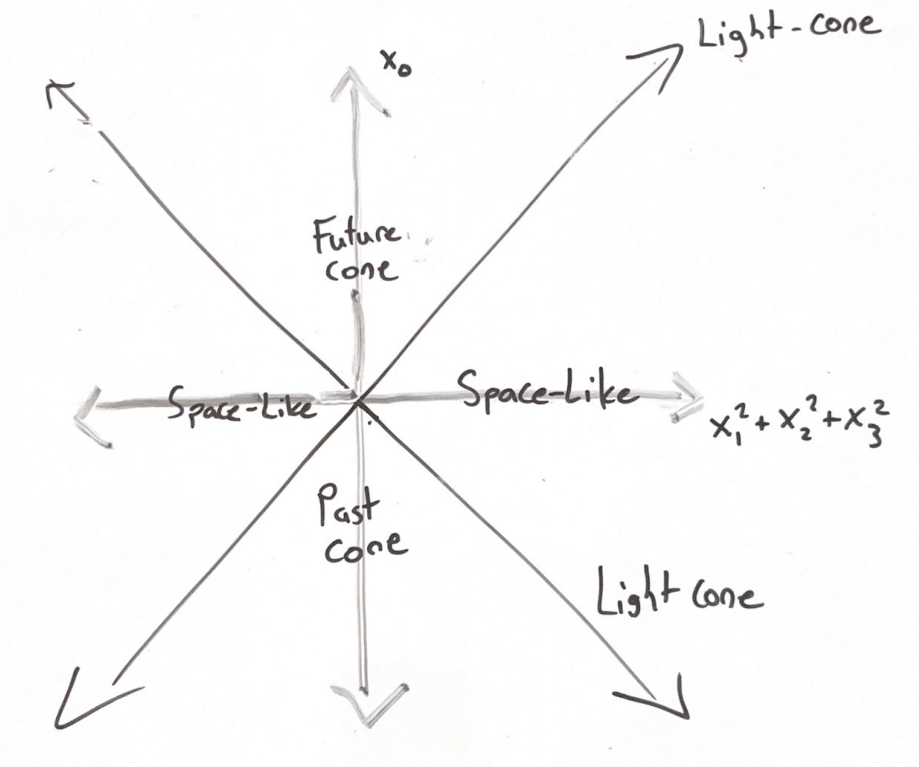
\includegraphics[width=0.5\textwidth]{Light cone-1}
	\caption{Decomposition of Minkowski Space based on length}
\end{figure}
\vfill
\end{frame}
%
%
\begin{frame}
\vfill
Useful Identity in $\overset{\sim}{L}_+$:
\begin{theorem}
	Any $\Lambda \in \overset{\sim}{L}_+$ can be uniquely written in the following way:
$$\Lambda = R(\theta,\phi,0)L_z(\xi)R(\alpha,\beta,\gamma)^{-1}$$
where $L_z(\xi)$ is a Lorentz boost along the $z$-axis by angle $\xi$ and the parameters for the Euler angles of the rotations from $SO(3)$ are defined as expected.
\end{theorem}
\vfill
Putting the Lorentz group together with $T_4$ gives us a new structure to study:
\vfill
\begin{definition}
	The set of all compositions of translations proper homogeneous Lorentz transformations is called the \textbf{Poincar\'e Group}, denoted $\overset{\sim}{P}$
\end{definition}
\end{frame}

\begin{frame}
\vfill
All transformations in the Poincar\'e group can be written as
\begin{equation}
\begin{aligned}
\begin{bmatrix}
	\underset{4\times 4}{\Lambda} & \underset{4\times 1}{b}\\
	\underset{1\times 4}{0} & \underset{1\times 1}{1}
\end{bmatrix}
\end{aligned}
\end{equation}
\vfill
Some Useful Identities:
\vfill
\begin{theorem}
For any $g(\Lambda,b)\in\overset{\sim}{P}$
\begin{equation}
\begin{aligned}
g(\Lambda,b)=T_b\Lambda
 \end{aligned}
\end{equation}
\end{theorem}
\vfill
\begin{theorem}
For any $\Lambda \in\overset{\sim}{L}_+$ and $T_b\in T_4$,
\begin{equation}
\begin{aligned}
	\Lambda T_b \Lambda^{-1} = T_{\Lambda b}
\end{aligned}
\end{equation}
\end{theorem}
\end{frame}
%
%
\begin{frame}
\vfill
In the pursuit of generators, we find the natural choices
\vfill
\begin{center}
\begin{tabular}{cc}
	$P_t = \begin{bmatrix}
				0 & 0 & 0 & 0 & i \\
				0 & 0 & 0 & 0 & 0\\
				0 & 0 & 0 & 0 & 0\\
				0 & 0 & 0 & 0 & 0\\
				0 & 0 & 0 & 0 & 0\\
			\end{bmatrix}$ &
	$P_x = \begin{bmatrix}
				0 & 0 & 0 & 0 & 0 \\
				0 & 0 & 0 & 0 & i\\
				0 & 0 & 0 & 0 & 0\\
				0 & 0 & 0 & 0 & 0\\
				0 & 0 & 0 & 0 & 0\\
			\end{bmatrix}$ \\
	$P_y = \begin{bmatrix}
				0 & 0 & 0 & 0 & 0 \\
				0 & 0 & 0 & 0 & 0\\
				0 & 0 & 0 & 0 & i\\
				0 & 0 & 0 & 0 & 0\\
				0 & 0 & 0 & 0 & 0\\
			\end{bmatrix}$ &
	$P_z = \begin{bmatrix}
				0 & 0 & 0 & 0 & 0 \\
				0 & 0 & 0 & 0 & 0\\
				0 & 0 & 0 & 0 & 0\\
				0 & 0 & 0 & 0 & i\\
				0 & 0 & 0 & 0 & 0\\
			\end{bmatrix}$
\end{tabular}
\end{center}
\vfill
\end{frame}


\begin{frame}
\vfill
\begin{center}
\begin{tabular}{ccc}
	$J_x = \begin{bmatrix}
				0 & 0 & 0 & 0 & 0 \\
				0 & 0 & 0 & 0 & 0\\
				0 & 0 & 0 & -i & 0\\
				0 & 0 & i & 0 & 0\\
				0 & 0 & 0 & 0 & 0\\
			\end{bmatrix}$ &
	$J_y = \begin{bmatrix}
				0 & 0 & 0 & 0 & 0 \\
				0 & 0 & 0 & i & 0\\
				0 & 0 & 0 & 0 & 0\\
				0 & -i & 0 & 0 & 0\\
				0 & 0 & 0 & 0 & 0\\
			\end{bmatrix}$ &
	$J_z = \begin{bmatrix}
				0 & 0 & 0 & 0 & 0 \\
				0 & 0 & -i & 0 & 0\\
				0 & i & 0 & 0 & 0\\
				0 & 0 & 0 & 0 & 0\\
				0 & 0 & 0 & 0 & 0\\
			\end{bmatrix}$ 
\end{tabular}
\end{center}
\vfill
And where $K_\mu$ is the generator for the Lorentz Boost along the $\mu$-axis.
\begin{center}
\begin{tabular}{ccc}
	$K_x = \begin{bmatrix}
				0 & i & 0 & 0 & 0 \\
				i & 0 & 0 & 0 & 0\\
				0 & 0 & 0 & 0 & 0\\
				0 & 0 & 0 & 0 & 0\\
				0 & 0 & 0 & 0 & 0\\
			\end{bmatrix}$ &
	$K_y = \begin{bmatrix}
				0 & 0 & i & 0 & 0 \\
				0 & 0 & 0 & 0 & 0\\
				i & 0 & 0 & 0 & 0\\
				0 & 0 & 0 & 0 & 0\\
				0 & 0 & 0 & 0 & 0\\
			\end{bmatrix}$ &
	$K_z = \begin{bmatrix}
				0 & 0 & 0 & i & 0 \\
				0 & 0 & 0 & 0 & 0\\
				0 & 0 & 0 & 0 & 0\\
				i & 0 & 0 & 0 & 0\\
				0 & 0 & 0 & 0 & 0\\
			\end{bmatrix}$ 
\end{tabular}
\end{center}
\vfill
\end{frame}

%
\begin{frame}
\vfill
\begin{equation}
\begin{aligned}
	\Lambda (\omega) = e^{-i\omega_1J_x}e^{-i\omega_2J_y}e^{-i\omega_3J_x}e^{-i\omega_4K_x}e^{-i\omega_5K_y}e^{-i\omega_6K_z}
\end{aligned}
\end{equation}
\vfill
Too many commutator relationships to be concise.
\vfill
We define one Casimir operator to be as excpected 
\begin{equation}
\begin{aligned}
	\mathfrak{C}_1 \coloneq \mathfrak{P}_t^2 -  \mathfrak{P}_x^2 -\mathfrak{P}_y^2- \mathfrak{P}_z^2
\end{aligned}
\end{equation}
If $\psi$ is an irreducible representation, then we want to treat the eigenvalue of $\psi_{\mathfrak{C}_1}$ by cases in order to calculate every unitary irreducible representaion. If the eigenvalue is $\lambda$, we will calculate the representations in the case when $\lambda >0$. 
\vfill
\end{frame}


\begin{frame}
\vfill
In this case, vectors must be time-like.
\vfill
Choosing starting vector $v_0\colon (\sqrt(\lambda),0,0,0)$. Our quotient group will be  $\overset{\sim}{P}/T_4 $. Little group: $SO(3)$.
\vfill
Representations are indicated by $s$, a half or whole integer (from $SO(3)$).  Explicitly,
\begin{equation}
\begin{aligned}
	\psi_{\mathfrak{J}^2} (v_0)_m = s(s+1)(v_0)_m
\end{aligned}
\end{equation}
\begin{equation}
\begin{aligned}
	\psi_{\mathfrak{J}_z} (v_0)_m = m(v_0)_m
\end{aligned}
\end{equation}
\begin{equation}
\begin{aligned}
	\psi_{\mathfrak{P}_\mu} (v_0)_m = \begin{cases}
										\sqrt{\lambda_1} & \text{if } \mu=t\\
										0 & \text{else}
										\end{cases}
\end{aligned}
\end{equation}
where $\alpha,\beta$ are the cylindrical angles of the 
\end{frame}
%
%
\begin{frame}
\vfill
We transform this starting vector with Lorentz transformations:
\begin{equation}
\begin{aligned}
	v_p\coloneq H_p((v_0)_m) = R(\alpha,\beta,0)L_z(\xi)(v_0)_m
\end{aligned}
\end{equation}
where $\alpha,\beta$ are the cylindrical angles of the vector $v_p$.
\vfill
\begin{theorem} Time-like Unitary Irreducible Representations of $\overset{\sim}{P}$
	The subspace generated by the vectors $\{(v_p)_m\}_{p,m}$ is invariant under $\overset{\sim}{P}$. The irreducible, unitary representations of elements of this group are characterized in the following way:
$$\psi_{T_b} (v_p)_m = e^{-ib_0p_0}e^{-ib_1p_1}e^{-ib_2p_2}e^{-ib_3p_3}(v_p)_m$$
$$\psi_\Lambda (v_p)_m = [\phi_s(H(p')\Lambda H(p))]_{m'm} (v_{p'})_{m'}$$
where $p' = \Lambda p$ and $\phi_s$ is the irreducible representation of $SO(3)$ defined by $s$.
\end{theorem}
\end{frame}

\section{Braid Group and Anyons}
\begin{frame}
\sectionpage
\end{frame}
%
%
\begin{frame}
\vfill
\begin{definition}
	The braid group, $B_n$, is generated by $n-1$ generators (denoted $\sigma_1,\hdots,\sigma_{n-1}$) that have the following "braid relations":
$$\sigma_i\sigma_j = \sigma_j\sigma_i \hspace{3mm} \forall i,j \in \{1,\hdots,n-1\} \text{ where } |i-j|>1$$
$$\sigma_i\sigma_{i+1}\sigma_i=\sigma_{i+1}\sigma_i\sigma_{i+1} \hspace{3mm} \forall i \in \{1,\hdots,n-2\}$$
\end{definition}
\vfill
\begin{definition}
	A \textbf{geometric braid} on $n\in \N$ strands is a set $b\subset\R^2\times [0,1]$ formed by $n$ disjoint, intervals topologically equivalent to $[0,1]$ such that we can define a projection mapping from $\R^2\times [0,1]$ to $[0,1]$ that maps each strand homeomorphically to $[0,1]$ and the following conditions hold:
$$b\cap(\R^2\times\{0\}) = \{(1,0,0),(2,0,0),\hdots,(n,0,0)\}$$
$$b\cap(\R^2\times\{1\}) = \{(1,0,1),(2,0,1),\hdots,(n,0,1)\}$$
\end{definition}
\vfill
\end{frame}


\begin{frame}
\vfill
\begin{figure}[H]
	\centering
	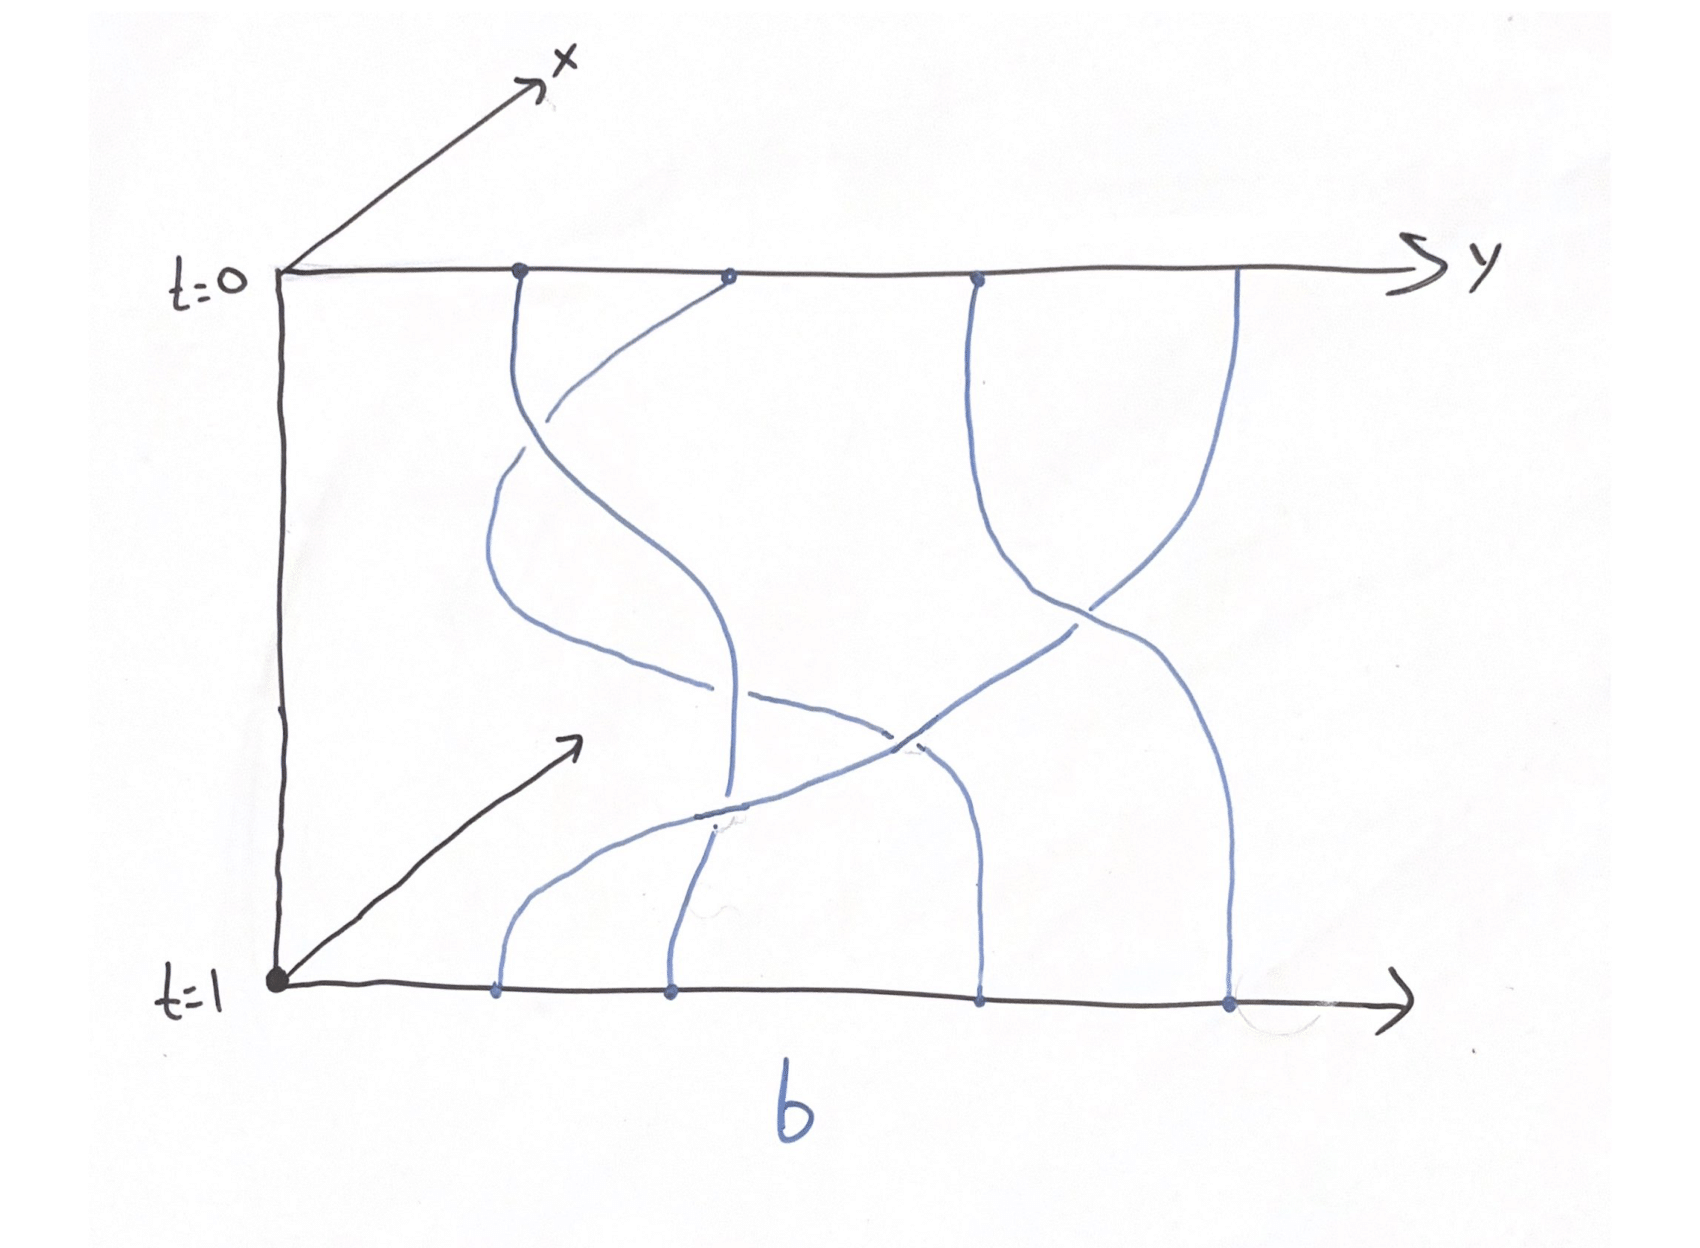
\includegraphics[width=0.5\textwidth]{geobraid.png}
	\caption{Generic geometric braid}
\end{figure}
\vfill
\begin{definition}
	Two braids, $b_1$ and $b_2$, are said to be \textbf{isotopic} to each other if one can be continuously deformed into the other. This is an equivalence relation.
\end{definition}
\vfill
\end{frame}
%
%
\begin{frame}
\vfill
\begin{equation}
\begin{aligned}
	b_1b_2 \coloneq \{(x,y,t)\mid (x,y,2t)\in b_1 \text{ when }0\leq t\leq \frac{1}{2} \text{ and }   (x,y,2t - 1)\in b_2 \text{ when }\frac{1}{2}\leq t\leq 1\}
\end{aligned}
\end{equation}
\vfill
\begin{figure}[H]
	\centering
	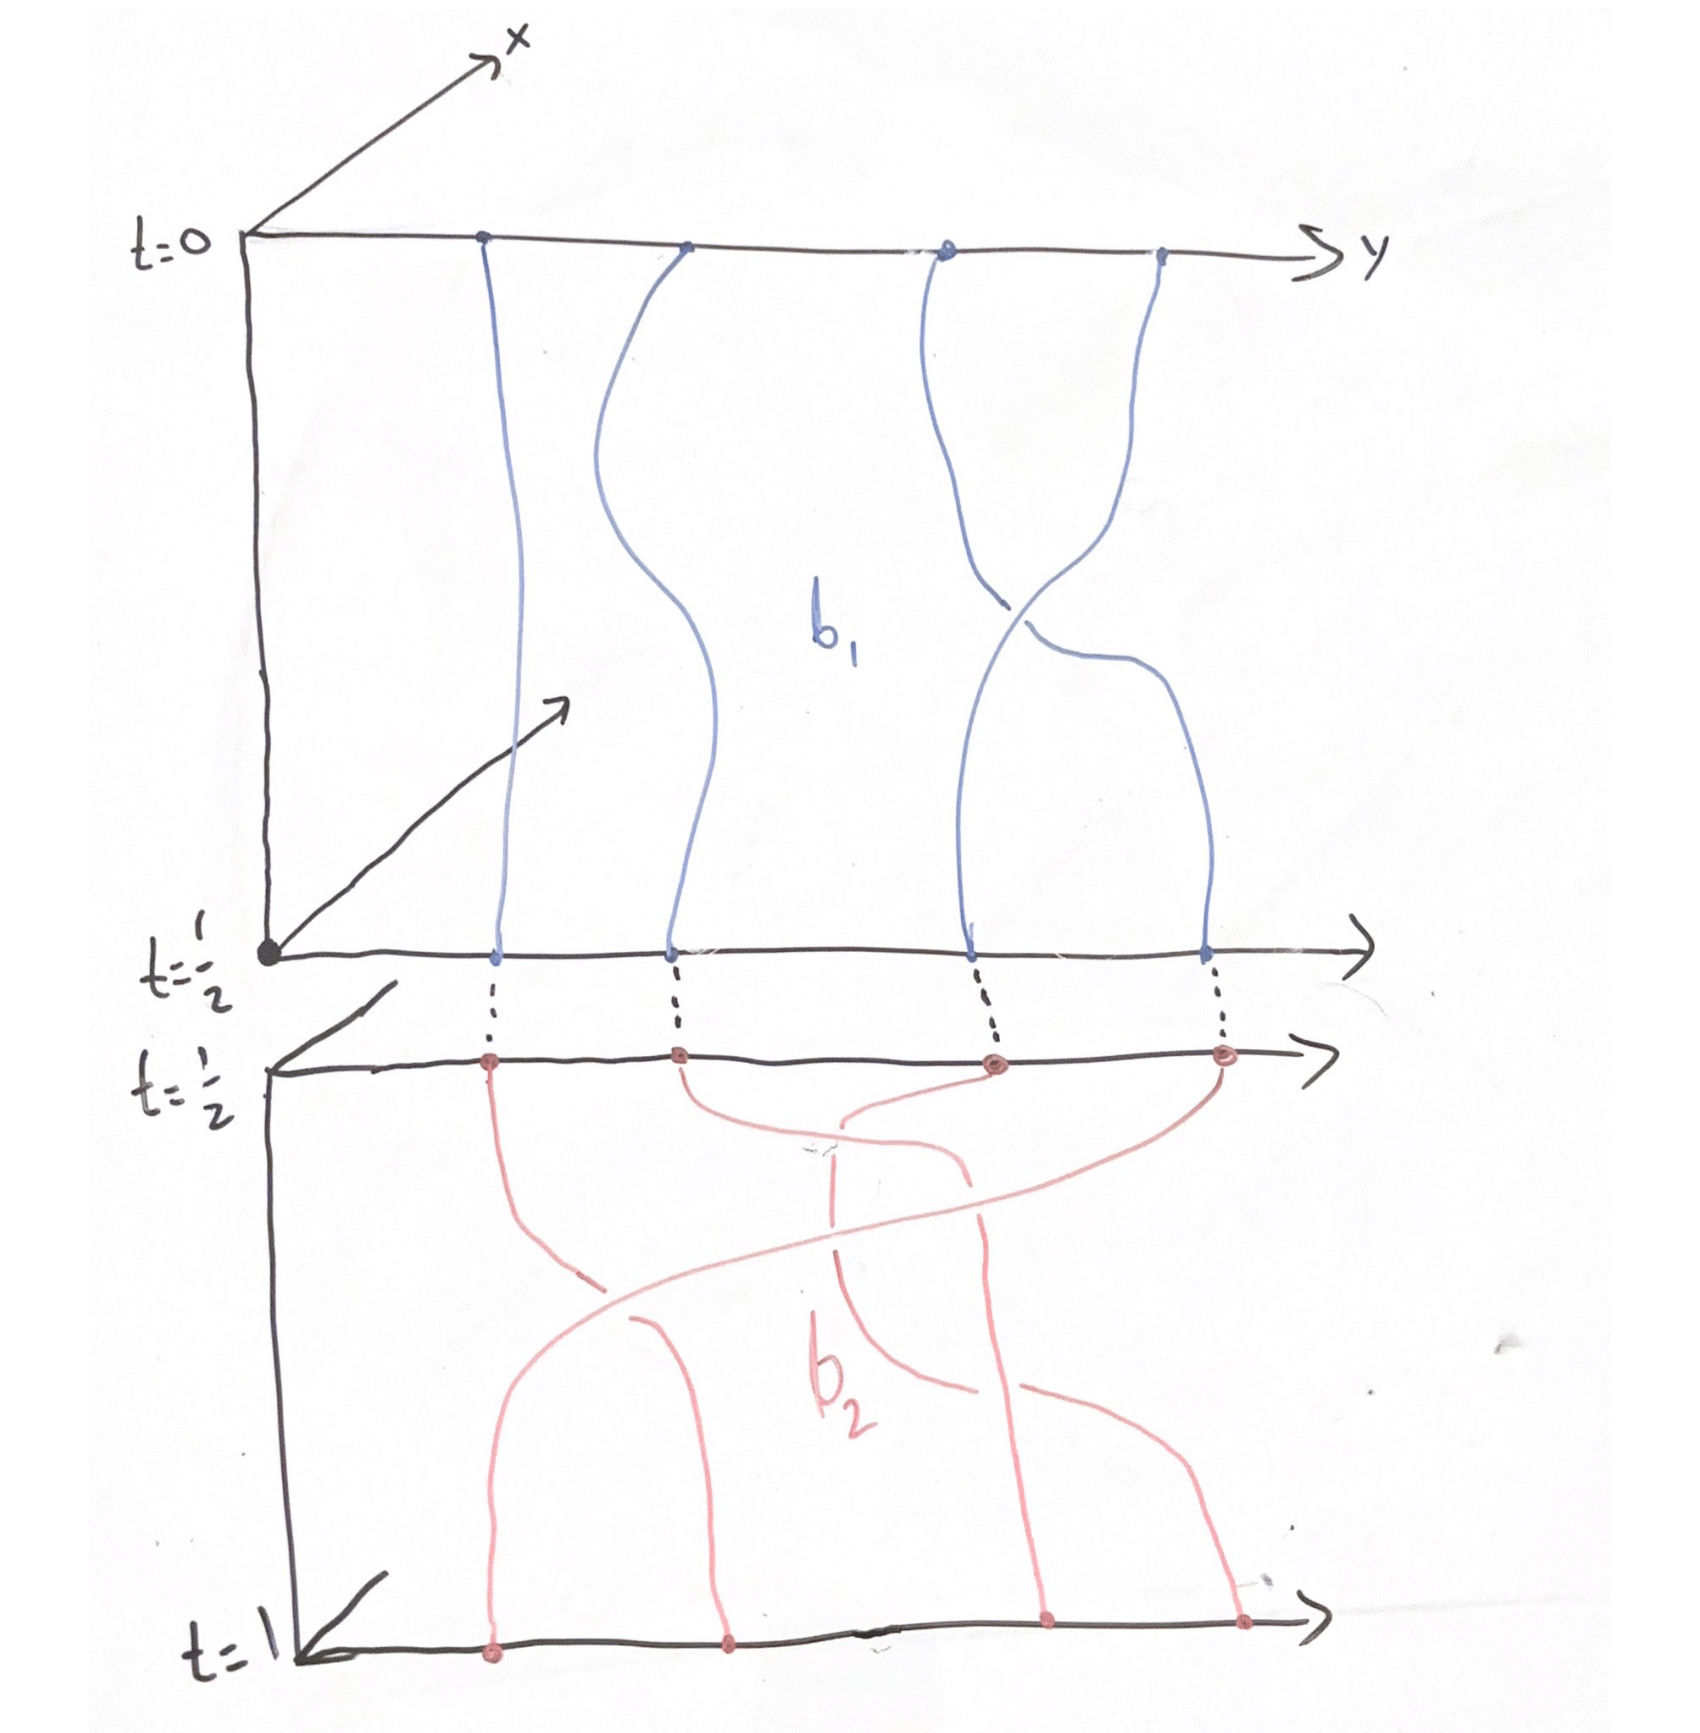
\includegraphics[width=0.3\textwidth]{geobraidprod.png}
	\caption{The product of two geometric braids.}
\end{figure}
\vfill
\end{frame}


\begin{frame}
\vfill
\begin{definition}
	A \textbf{braid diagram} on $n$ strands is set, $\mathcal{D}\subset \R\times [0,1]$ made up as a union of $n$ intervals topologically equivalent to $[0,1]$ (called strands) such that the following conditions are met:
\begin{itemize}
	\item There exists a projection map from $\R\times [0,1]$ to $[0,1]$ that maps each strand homeomorphically to $[0,1]$.
	\item Every element of $\{1,2,\hdots,n\}\times\{0,1\}$ is a starting or endpoint of a unique strand.
	\item Every element in $\mathcal{D}$ belongs to either one or two strands. When an elment belongs to two, one strand must be designated as overgoing and the other undergoing (referred to as a crossing of $\mathcal{D}$
\end{itemize}
\end{definition}
\vfill
While it is definitely true that every geometric braid has a braid diagram, the identification is not unique.
\end{frame}
%
%
\begin{frame}
\vfill
\begin{figure}[H]
	\centering
	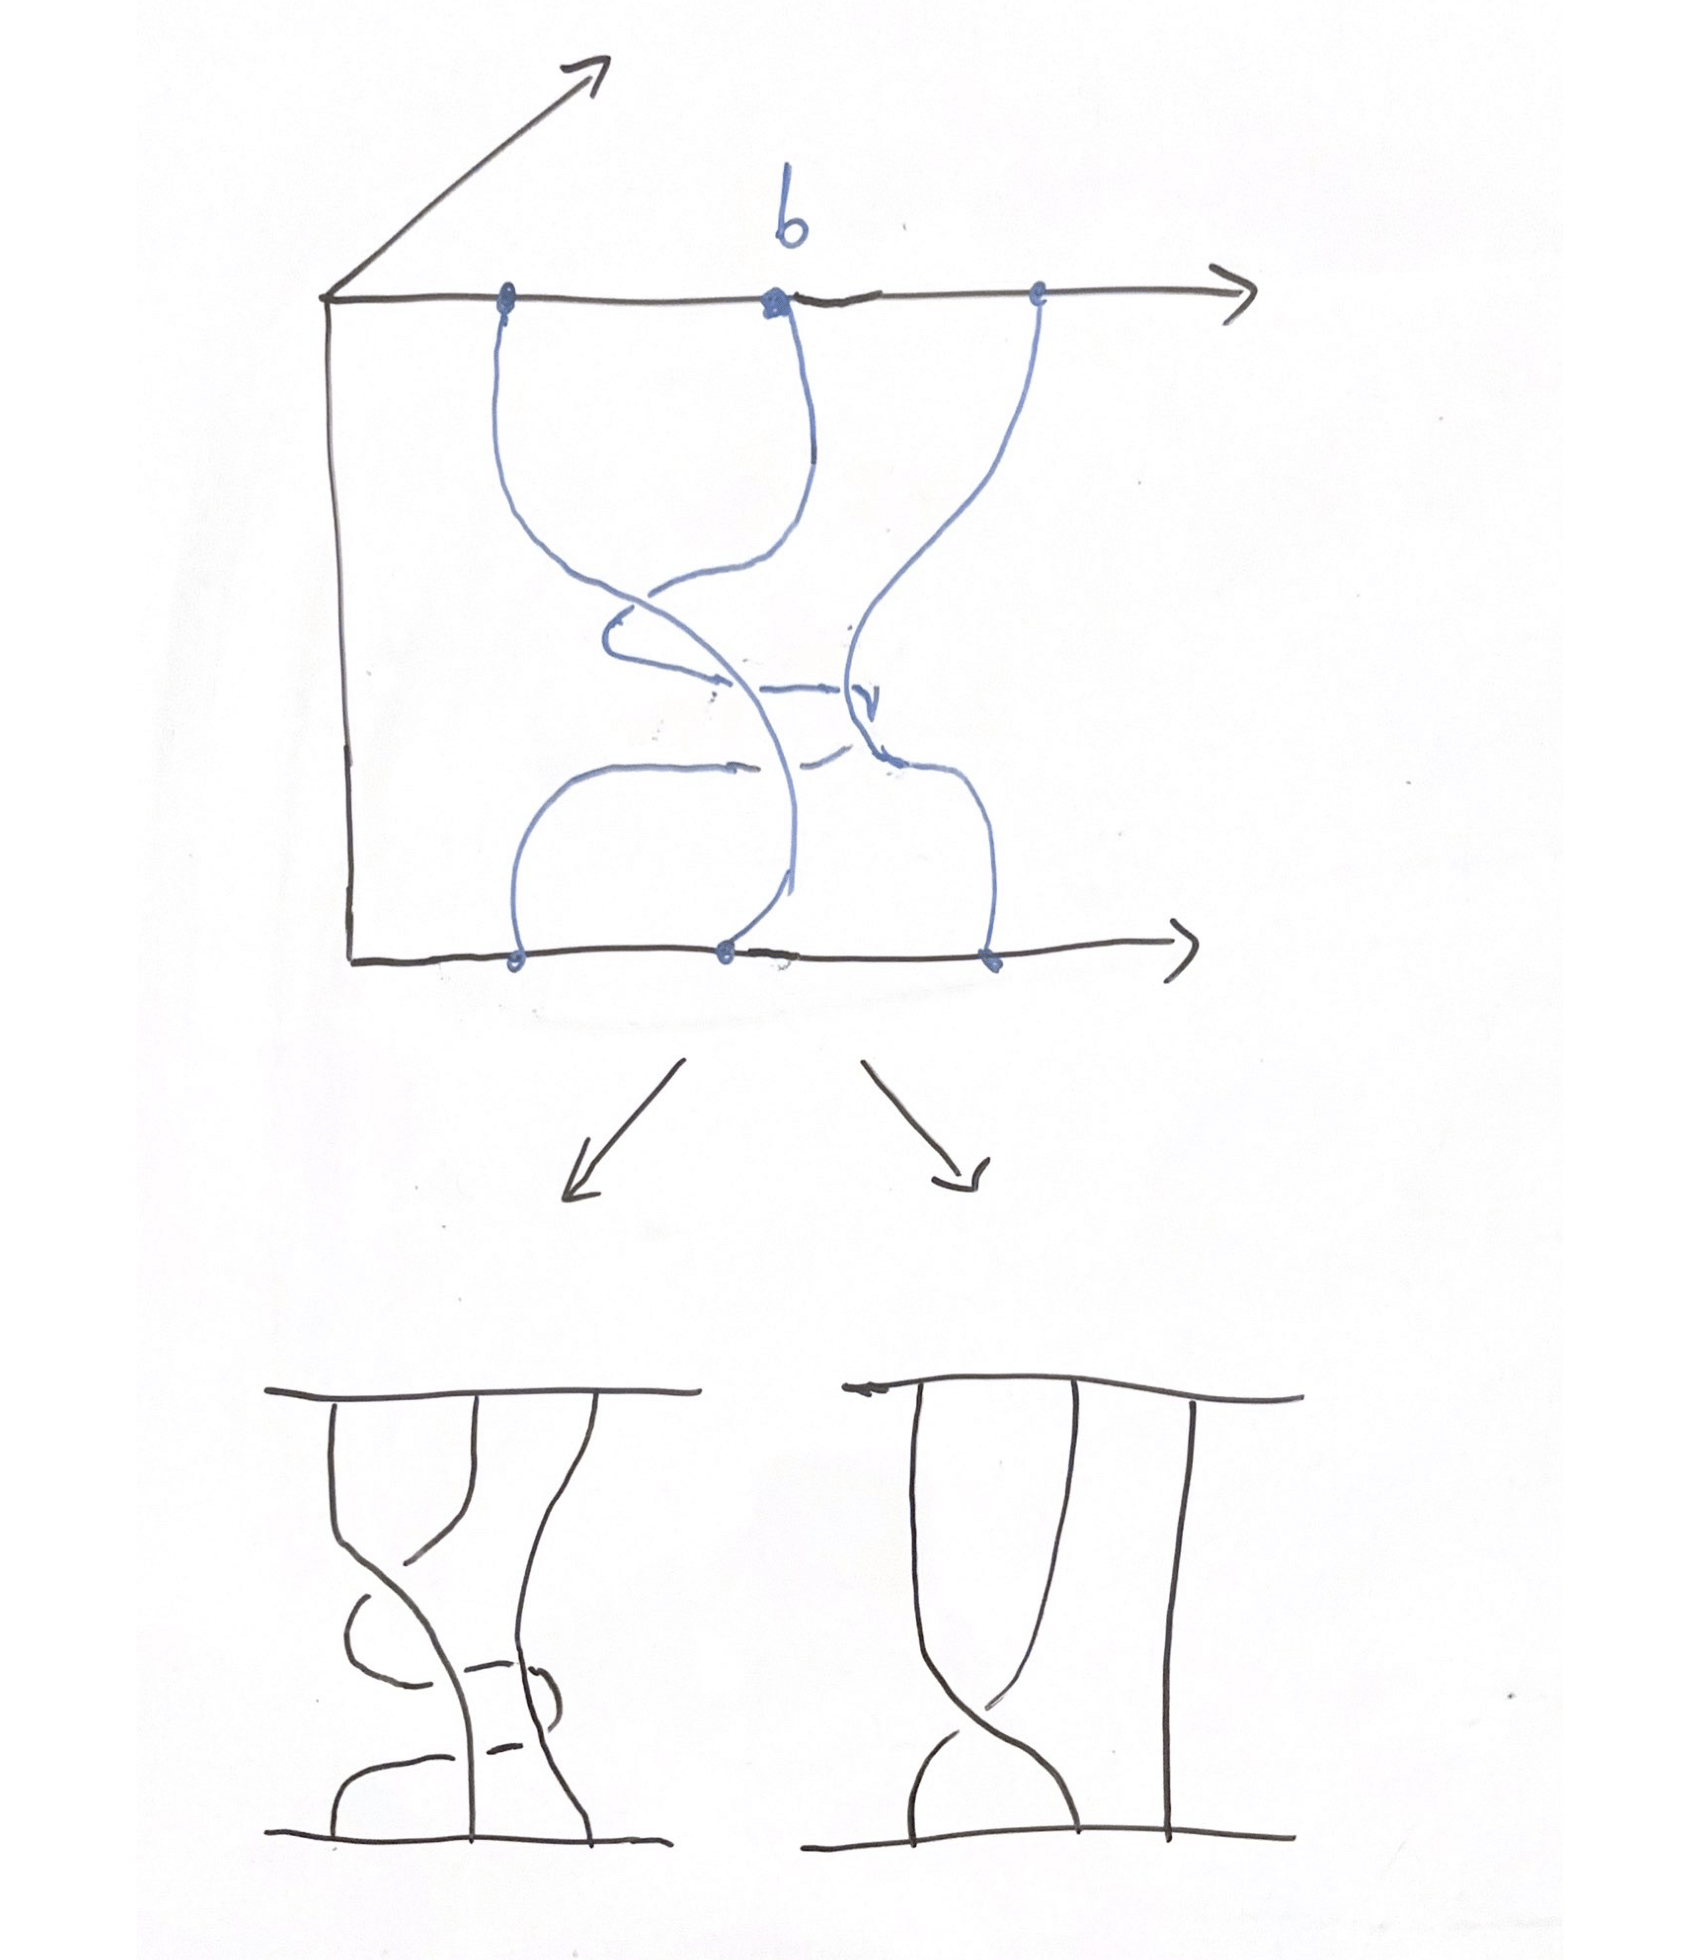
\includegraphics[width=0.5\textwidth]{requiv.png}
	\caption{Two braid diagrams that correspond to the same geometric braid.}
\end{figure}
\vfill
We can identify when braid diagrams represent the same braid with the following Reidemeister moves.
\end{frame}


\begin{frame}
\vfill
\begin{figure}[H]
	\centering
	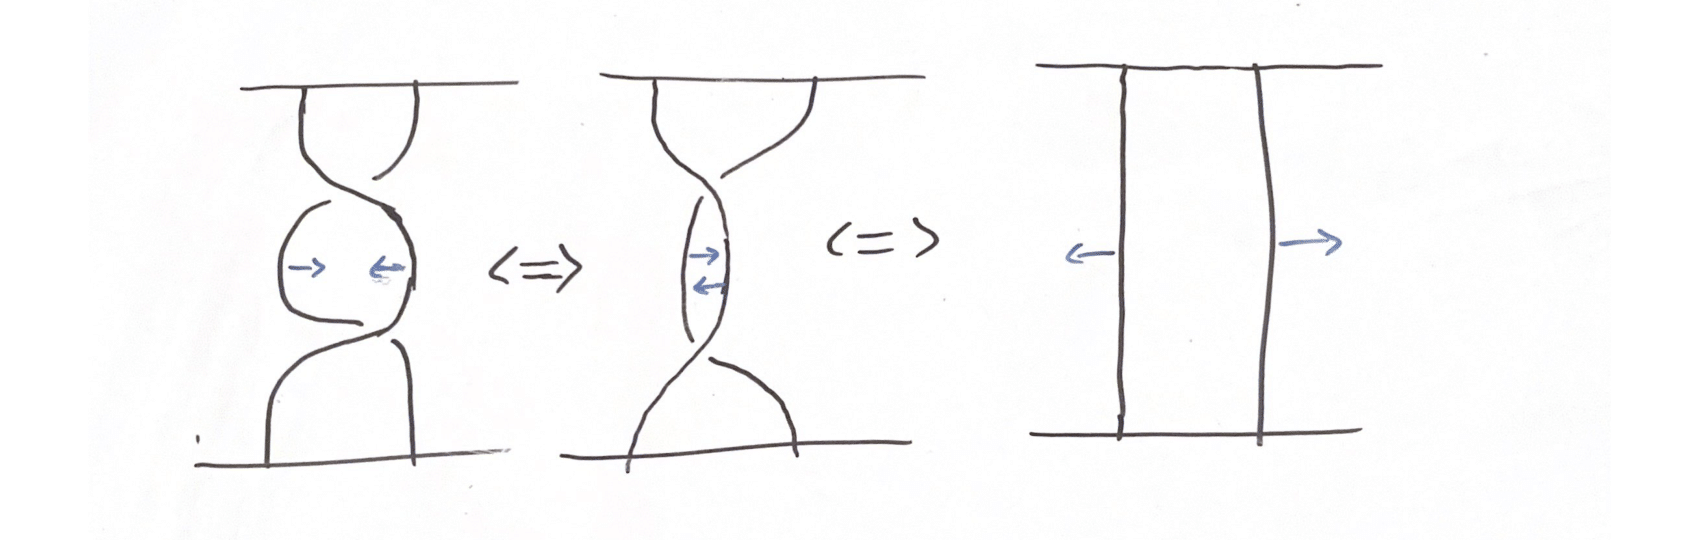
\includegraphics[width=0.7\textwidth]{reidmove2.png}
	\caption{$\Omega_1^{-1}$}
\end{figure}

\vfill
\begin{figure}[H]
	\centering
	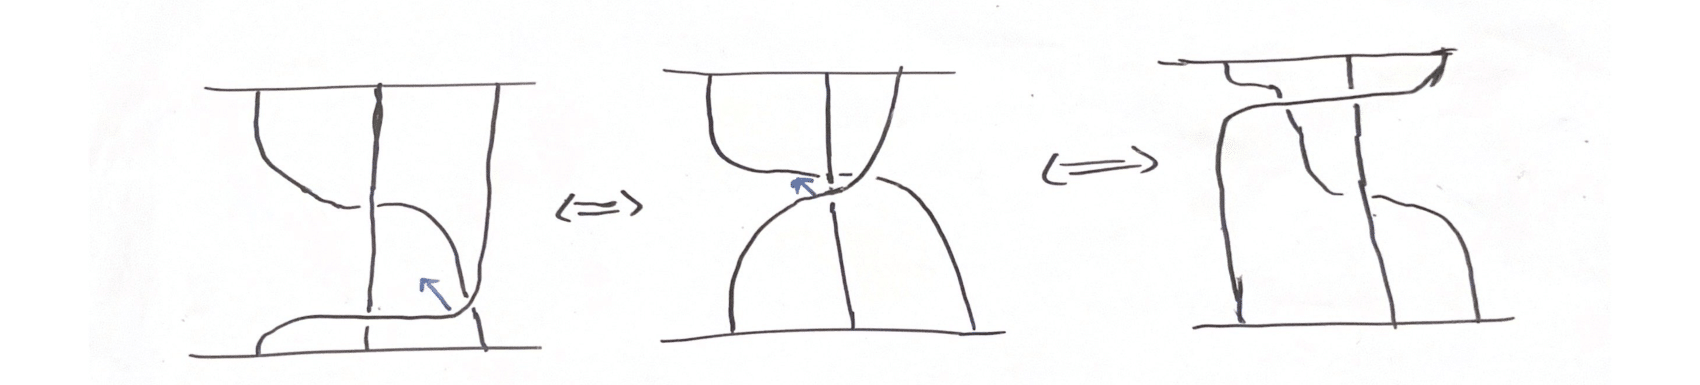
\includegraphics[width=0.7\textwidth]{reidmove3.png}
	\caption{$\Theta$}
\end{figure}
\end{frame}
%
%
\begin{frame}
\vfill
\begin{definition}
	Two braid diagrams are said to be \textbf{R-equivalent} if one can be transformed into the other by means of a finite sequence of isotopies and Reidemeister moves. This is an equivalence relation.
\end{definition}
\vfill
Braids can be decomposed in the following way:
\begin{theorem}
	Let $\mathcal{B}_n$ be the group of geometric braids on $n$ strands. Then for any $\beta\in\mathcal{B}_n$, $\beta$ has a natural decomposition:
$$\beta = \sigma_{i_1}\hdots\sigma_{i_k}$$ 
where $i_1,i_2,\hdots,i_k\in\{1,2,\hdots,n-1\}$.
\end{theorem}
\vfill
\end{frame}

\begin{frame}
\vfill
Now that we have characterized the group, we can discuss representations. We consider the ring of matrices over the ring $\Z[t,t^{-1}]$
\vfill
For $i\in\{1,\hdots,n-1\},n>1$, define
\begin{equation}
\begin{aligned}
U_i = \begin{bmatrix}
			I_{i-1}& 0 & 0 & 0 \\
			0 & 1-t & t & 0\\
			0 & 1 & 0 & 0\\
			0 & 0 & 0 & I_{n-i-1}
		\end{bmatrix}
\end{aligned}
\end{equation}
\vfill
\end{frame}


\begin{frame}
\vfill
\begin{definition}
	The \textbf{Burau Representation} of $B_n$ is the map 
$$\phi_n:B_n\rightarrow M_n(\Z[t,t^{-1}])$$
$$\sigma_i \mapsto U_i$$
\end{definition}
\vfill
If we compose this map with a ring homomorphism on $\Z[t,t^{-1}]$ that evaluates elements at some complex number with magnitude one, the result is a unitary representation.
\end{frame}
%
%
\begin{frame}
\vfill
Let us shift our discussion towards anyonic systems. In quantum mechanics, we study wave functions.
\vfill
\begin{equation}
	\begin{aligned}
		\int_\Omega |\psi|^2 d\mu = 1
	\end{aligned}
\end{equation}
\vfill
Wave function encodes information depending on inputs. For our purposes, inputs are positions.
\vfill 
Suppose we have a two particle system where particles are indistinguishable.
\vfill
\end{frame}


\begin{frame}
\vfill
After one particle exchange:
\begin{equation}
	\begin{aligned}
		\psi(r_1,r_2) = e^{i\theta} \psi(r_2,r_1) \hspace{3mm}\text{for some }\theta\in[0,2\pi)
	\end{aligned}
\end{equation}
\vfill
After two particle exchanges:
\begin{equation}
	\begin{aligned}
		\psi(r_1,r_2) = e^{2i\theta} \psi(r_1,r_2) \hspace{3mm}\text{for some }\theta\in[0,2\pi) \hspace{1mm} a.e.
	\end{aligned}
\end{equation}
\vfill
This means $\theta=0,\pi$: Bosons or Fermions.
\vfill
\end{frame}
%
%
\begin{frame}
\vfill
However, in two dimensions, it is not always the case that returning back to starting position returns our value. Rather, the anyons begin to braid. This is more clearly seen with $n$ anyons.
\vfill
We say that the particles obey $\theta$-statistics if the wave function picks up a factor of $e^{i\theta}$ upon exchange. Anyons obey $\theta$-statistics where $\theta\neq0,\pi$.
\vfill
Using this concept, we can build a degree one representations of $B_n$.
\end{frame}


\begin{frame}
\vfill
\begin{block}{Representation}
$$\phi_\theta:B_n\rightarrow \C$$
$$\beta\mapsto e^{i\theta}$$
\end{block}
\vfill
If $\beta\in B_n$ with decomposition $\beta = \sigma^{m_1}_{i_1}\hdots\sigma^{m_k}_{i_k}$ for some $i_1,\hdots,i_k\in\{1,\hdots,n-1\},m_j\in\N$, and if $\sigma$ is the underlying permutation of $\beta$, then
\begin{equation}
	\begin{aligned}
		\psi(\sigma(r_1),\sigma(r_2),\hdots,\sigma(r_n)) = e^{i\theta(m_1+\hdots+m_k)} \psi(r_1,r_2,\hdots,r_m)
	\end{aligned}
\end{equation}
\vfill
Since the image of this homomorphism is an abelian group, we say these anyons are abelian.
\end{frame}

%
\begin{frame}
\vfill
Another representation can be defined in the following way:
\begin{theorem}
	Let $V \coloneq \bigotimes_{i=1}^m\psi$ where $m>1$ and let $R: V\otimes V \rightarrow V\otimes V $ be an invertible, linear operator. Then the following map is a representation of $B_n$
$$\phi_R:B_n\rightarrow GL_m(\C)$$
$$\sigma_i \mapsto M(U_i)$$
where $M(U_i)$ is the matrix of the operator $U_i$ defined by
$$U_i:V\rightarrow V$$
$$(v_1\otimes\hdots\otimes v_i\otimes v_{i+1}\otimes\hdots\otimes v_m)\mapsto (v_1\otimes\hdots\otimes R(v_i\otimes v_{i+1})\otimes\hdots\otimes v_m)$$
\end{theorem}
\vfill
\begin{equation}
	\begin{aligned}
		M(U_i) = \begin{bmatrix}
						I_{i-1} & 0 & 0 \\
						0 & M(R) & 0 \\
						0 & 0 & I_{m - i - 1}
					\end{bmatrix}
	\end{aligned}
\end{equation}
\vfill
\end{frame}


\begin{frame}
\vfill
\begin{block}{Question}
What happens if anyons obey different statistics?
\end{block}
\vfill
We continue our work in the context of monoidal category theory
\vfill
\begin{definition}
	A monoidal category is a category, $C$, equipped with the following structure:
\begin{itemize}
	\item a bifunctor $\otimes:C\times C\rightarrow C$
	\item an object $e$ which acts as the identity object
	\item three natural isomorphisms defined in the following way:
		\begin{itemize}
			\item The associator, $\alpha$, whose components are $\alpha_{a,b,c}: a\otimes(b\otimes c) \cong (a\otimes b)\otimes c$
			\item The left unitor, $\lambda$, whose components are $\lambda_a : e\otimes a \cong a$
			\item The right unitor, $\rho$, whose components are $\rho_a:a\otimes e \cong a$
		\end{itemize}
\end{itemize}
\end{definition}
\vfill
\end{frame}
%
%
\begin{frame}
\vfill
\begin{figure}[H]
	\centering
	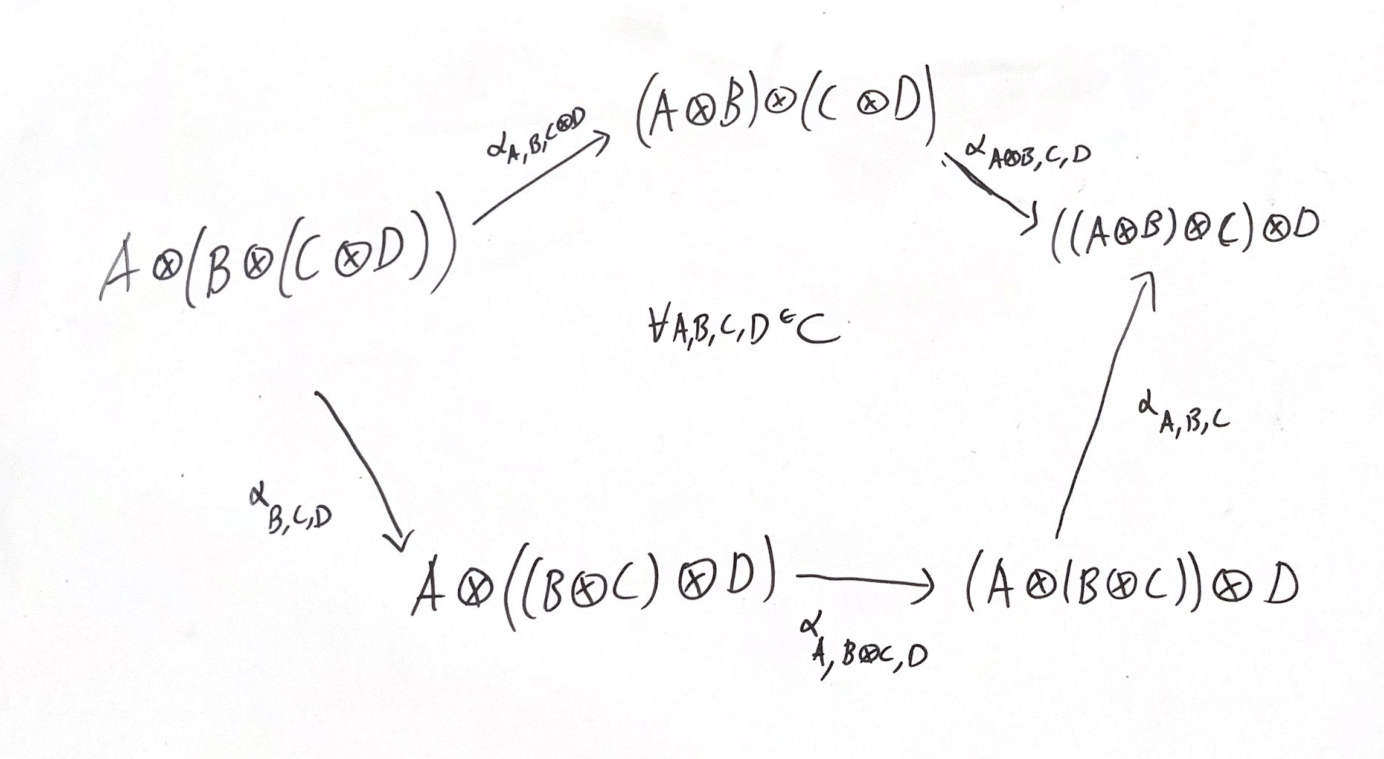
\includegraphics[width=0.7\textwidth]{pent diag.png}
	\caption{Commutative Pentagon Diagram for Monoidal Categories}
\end{figure}
\vfill
\end{frame}


\begin{frame}
\vfill
Here, the tensor product corresponds to the fusion of two anyons. We will be characterizing the Fibonacci anyonic system.
\vfill
If $e$ is the identity anyon type (vacuum), and $\tau$ is a nontrivial anyon type, then our system is characterized by this rule:
\begin{equation}
	\begin{aligned}
		\tau \otimes \tau = 1\oplus \tau
	\end{aligned}
\end{equation}
\vfill
We say that $\tau$ has multi-fusion channels. We represent all possible fushion paths in tree diagrams in the following way:
\vfill
\end{frame}
%

\begin{frame}
\vfill
\begin{figure}[H]
	\centering
	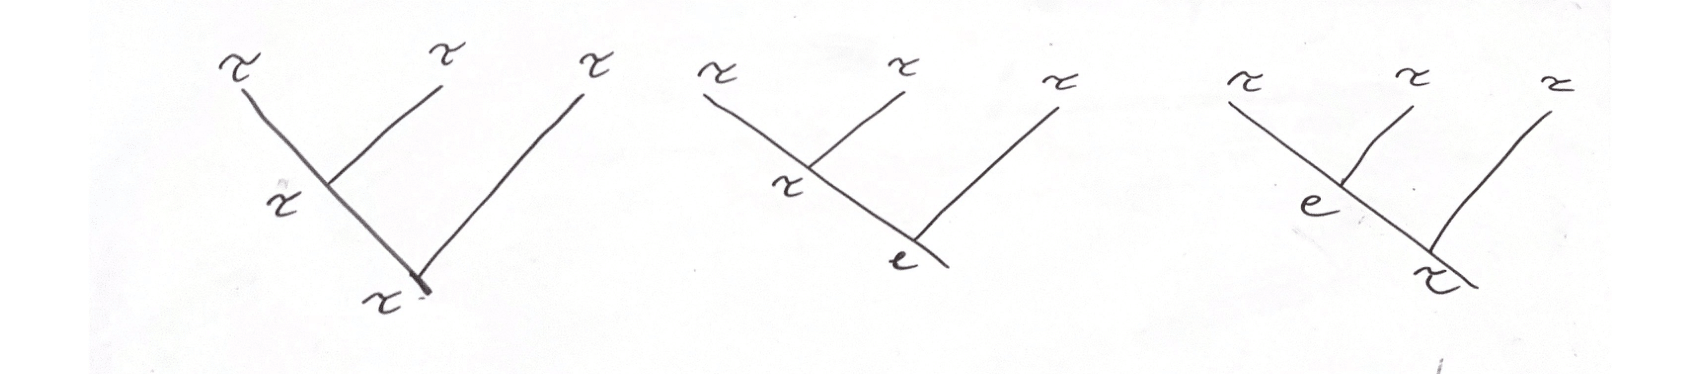
\includegraphics[width=1\textwidth]{treebasis.png}
	\caption{These tree diagrams are labelled according to the fusions rules of Fibonacci anyons.}
\end{figure}
\vfill
The Fibonacci sequence counts the number of fushion paths that can be taken. These fusion paths represent an orthonormal basis of some underlying vector space.
\end{frame}


\begin{frame}
\vfill
There is nothing to stop fushion from occuring in any order.
\vfill
\begin{figure}[H]
	\centering
	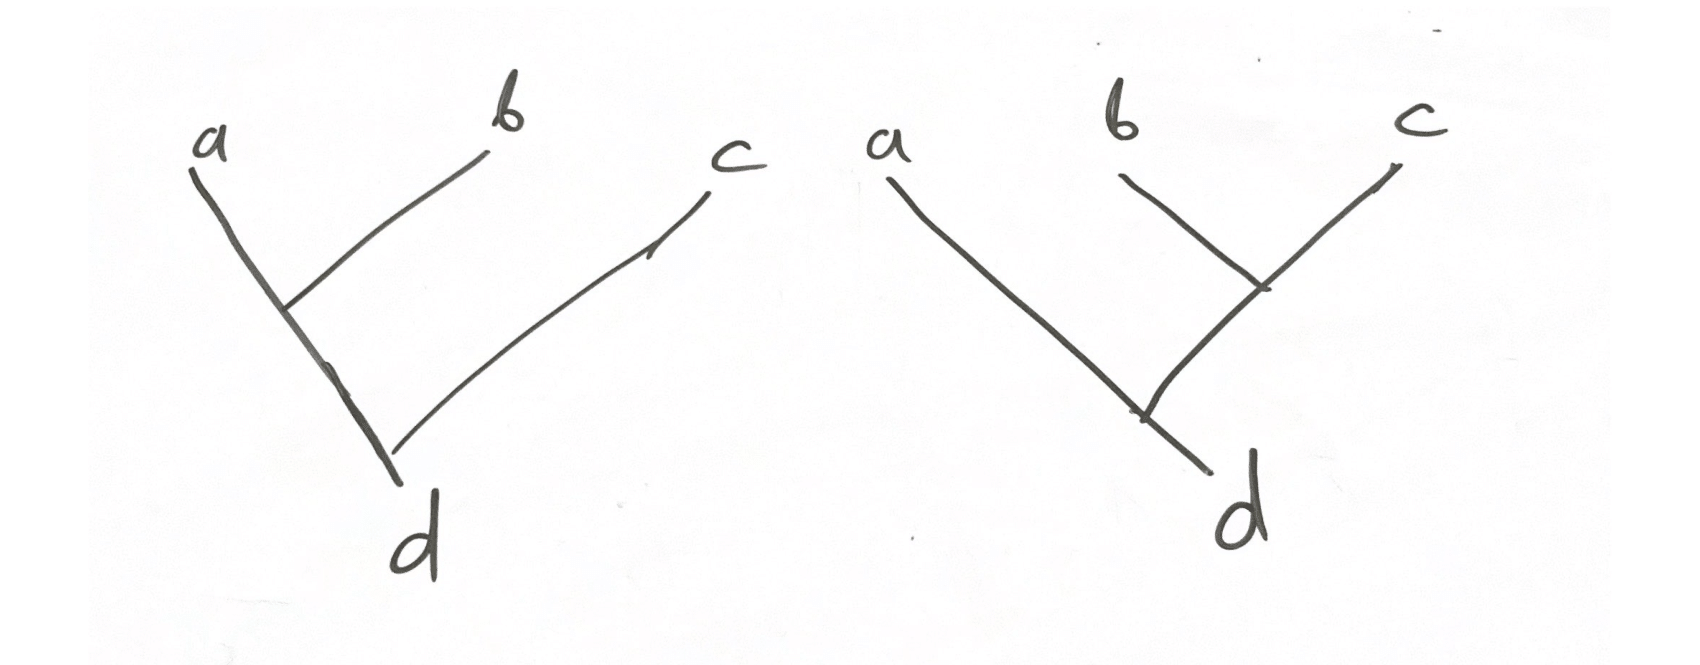
\includegraphics[width=0.7\textwidth]{differentftb}
	\caption{Both tree diagrams represent a different fusion order on the same anyon types.}
\end{figure}
\vfill
Transforming from one basis to another should be a linear, unitary operation, and as such can be depicted in a matrix. We call these transformations $F$-moves. Denote $F^{abc}_d$ as the $F$-move that moves $(a\otimes b)\otimes c$ to $a\otimes(b\otimes c)$ over total charge $d$.
\vfill
We use the commutative diagram to construct systems of equations to solve for each $F$ explicitly
\end{frame}
%
%
\begin{frame}
\vfill
$F^{abc}_d$ is the identity matrix if any the fusion associates any identity particles. Therefore, we must solve for $F^{\tau\tau\tau}_\tau$.
\vfill
\begin{equation}\begin{aligned}
[F^{\tau\tau\tau}_\tau]_{11} = [F^{\tau\tau\tau}_\tau]_{12}[F^{\tau\tau\tau}_\tau]_{21}
\end{aligned}\end{equation}
\vfill
\begin{equation}
	\begin{aligned}
		F^{\tau\tau\tau}_\tau = \begin{bmatrix}
									\frac{1}{\Phi} & \frac{1}{\sqrt{\Phi}}\\
									\frac{1}{\sqrt{\Phi}} & -\frac{1}{\Phi}
								\end{bmatrix}
	\end{aligned}
\end{equation}
where $\Phi$ is the golden ratio.
\vfill
\end{frame}


\begin{frame}
\vfill
Choosing to reintroduce braiding to the set up gives us the ability to embed ourselves in another kind of category: a Braiding Monoidal Category
\vfill
Here, braiding and fusion have to behave well with one another
\begin{figure}[H]
	\centering
	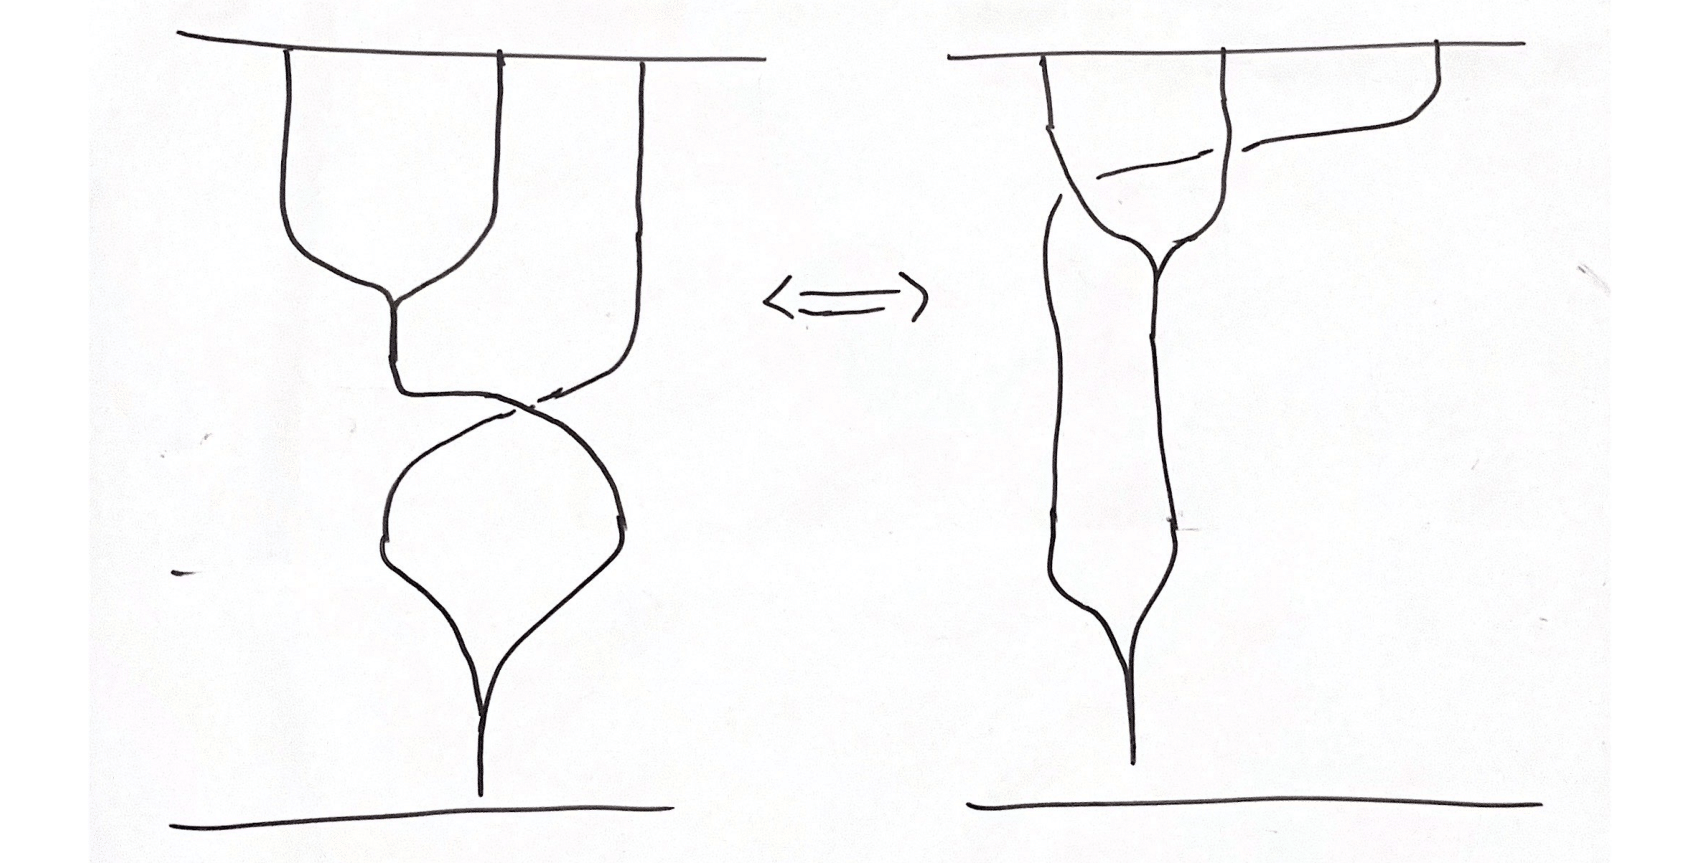
\includegraphics[width=0.7\textwidth]{fusethrubraid.png}
	\caption{Compatibility of braiding and fusion.}
\end{figure}
\vfill
\end{frame}
%
%
\begin{frame}
\vfill
Here, we refer to individual anyon exchanges as $R$-moves and these can be encoded into matrices due to their basis transforming abilities on our fusion paths. We take the convention that $R^{a,b}_c$ swaps $a$ and $b$ with total charge $c$ fused. We solve a similar system of equations to find explicit $R$ matrices
\vfill
\begin{equation}
	\begin{aligned}
		(R^{\tau,\tau}_e)^2\frac{1}{\Phi} = R^{\tau,\tau}_\tau\frac{1}{\Phi} + \frac{1}{\Phi^2}
	\end{aligned}
\end{equation}
\begin{equation}
	\begin{aligned}
		R^{\tau,\tau}_eR^{\tau,\tau}_\tau\frac{1}{\sqrt{\Phi}} = (1-R^{\tau,\tau}_\tau)\frac{1}{\Phi^\frac{3}{2}} 
	\end{aligned}
\end{equation}
\begin{equation}
	\begin{aligned}
		-(R^{\tau,\tau}_e)^2\frac{1}{\Phi} = R^{\tau,\tau}_\tau\frac{1}{\Phi^2}+\frac{1}{\Phi}
	\end{aligned}
\end{equation}
\end{frame}


\begin{frame}
\vfill 
It is difficult to find solutions to these equations in general. If we make the assumption that our state space is one dimensional, these matrices should be one dimensional with values $R^{\tau\tau}_e = e^{i\frac{4\pi}{5}}$ and $R^{\tau\tau}_\tau = e^{i\frac{-3\pi}{5}}$.
\vfill
In order to encode a true braiding effect in this set up, we need to ensure that the braid takes into account fusions. Braiding matrices take the following form:
\begin{equation}
	\begin{aligned}
		B = F^{-1}R F
	\end{aligned}
\end{equation}
\vfill
We need more specificity to the scenario to calculate a specific solution for this set up.
\end{frame}
%
%
\begin{frame}
\vfill
\begin{figure}[H]
	\centering
	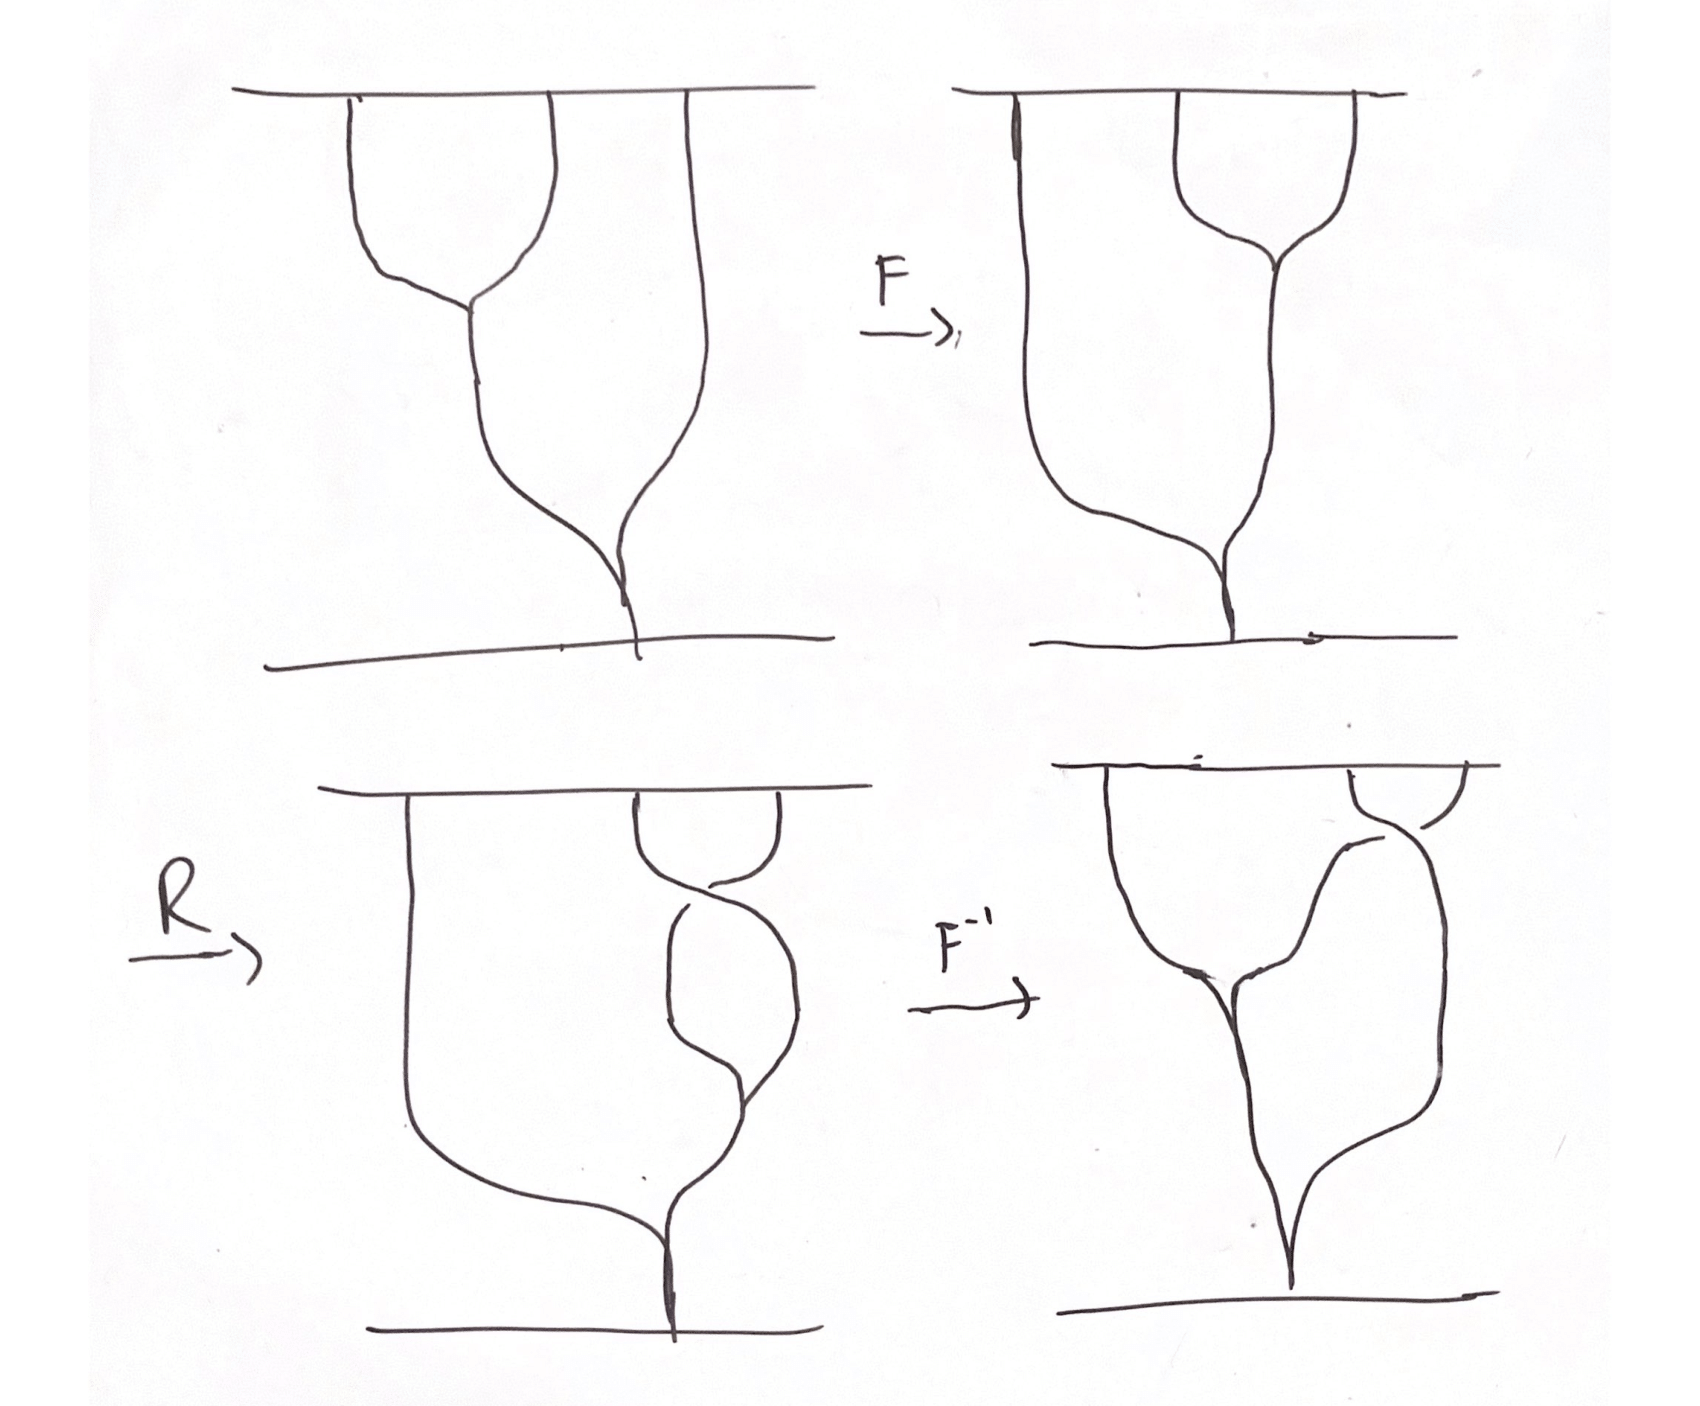
\includegraphics[width=0.7\textwidth]{braid.png}
	\caption{The process of braiding decomposed into fusion and anyon exchanges.}
\end{figure}
\vfill 

\end{frame}


\begin{frame}
\vfill
Thank You
\vfill
\end{frame}


%\begin{frame}
%\vfill
%\vfill
%\end{frame}




\end{document}